\section{Multi-Agent Path Finding}
\label{sec:MAPF}
The \acrf{mapf} problem is the problem of planning a feasible path for multiple
agents~\cite{MAPF_definitions}:
\begin{definition}[\acrl{MAPF}]
  Given a graph $G=(V,E)$, a function $S$ that maps the agents to their initial
  positions and a function $E$ that maps the agents to the their final
  positions, the problem amounts to finding a feasible joint plan $\Pi$ such
  that each agent reaches its destination, while globally minimizing an
  objective function.
\end{definition}
A joint plan $\Pi$ is the set of the individual plans $\pi_i$ that each agent
$a_i$ has to follow to reach its destination: 
\[\Pi=\{\pi_1, \hdots, \pi_k\}\]
There are different definitions of the problem in terms of how the graph 
topology is assumed to be, but the classical one
considers~\cite{MAPF_definitions}:
\begin{itemize}
  \item $G$ is an \textit{undirected} graph;
  \item A node (or vertex) can host only one agent at the time;
  \item The edges between nodes have a binary value, either there is a
    connection and it costs 1, or there is no connection;
  \item It follows that time is assumed to be discretized into timestamps: at
    each time the agent can either move to a neighbor or stay on the node it is
    on. 
\end{itemize}
A joint plan $\Pi$ is simply the set of the paths that each agent needs to
follow to reach its goal, and it is said to be feasible if no conflict 
happens between different agents. In literature, there are different 
definitions of conflict, but the most important ones are the 
following~\cite{MAPF_overview}: 
\begin{itemize}
  \item \textit{Vertex conflict}: when two agents $a_i$ and $a_j$ are on the 
    same node at the same time $t$ (Figure~\ref{fig:vertexConflict}):
    \[\pi_i(t) = \pi_j(t) \iff \text{vertex conflict}\]
  \item \textit{Edge conflict}: when two agents $a_i$ and $a_j$ move on the 
    same edge in the same direction at the same time $t$;
    \[\pi_i(t) = \pi_j(t) \wedge \pi_i(t+1) = \pi_j(t) \iff \text{edge 
      conflict}\]
  \item \textit{Swap conflict}: when two agents $a_i$ and $a_j$ are moving on 
    the same edge, but in different directions at the same time $t$
    (Figure~\ref{fig:swapConflict}). 
    \[\pi_i(t) = \pi_j(t+1) \wedge \pi_i(t+1) = \pi_j(t) \iff \text{swap 
      conflict}\]
\end{itemize}
Given the definition of vertex conflict, it follows that in the classical
definition of \acrs{mapf}, the edge conflict is avoided a priori by imposing
the absence of vertex conflicts since since two agents at time $t$ must have
different positions. For this reason, the terms edge conflict and swap conflict
may be used to indicate the same conflict in this work. \newline
Another type of conflict is the \textit{follow conflict}, shown in
Figure~\ref{fig:followConflict} which happens when an agent wants to occupy a
position at time $t$ that was occupied by another agent at time $t-1$. This
is particularly interesting for an industrial scenario since a follow conflict
may lead to delays or even collisions. Indeed, when an agent stops at a goal
point to be loaded, it may undergo some delays leading to possible problems for
the other agent following up. In this work, the following conflict will not be
taken into consideration as it is not strictly part of the classical
\acrs{mapf} problem.
\begin{figure}[tb]
  \centering
  \begin{subfigure}[t]{0.3\linewidth}
    \centering
    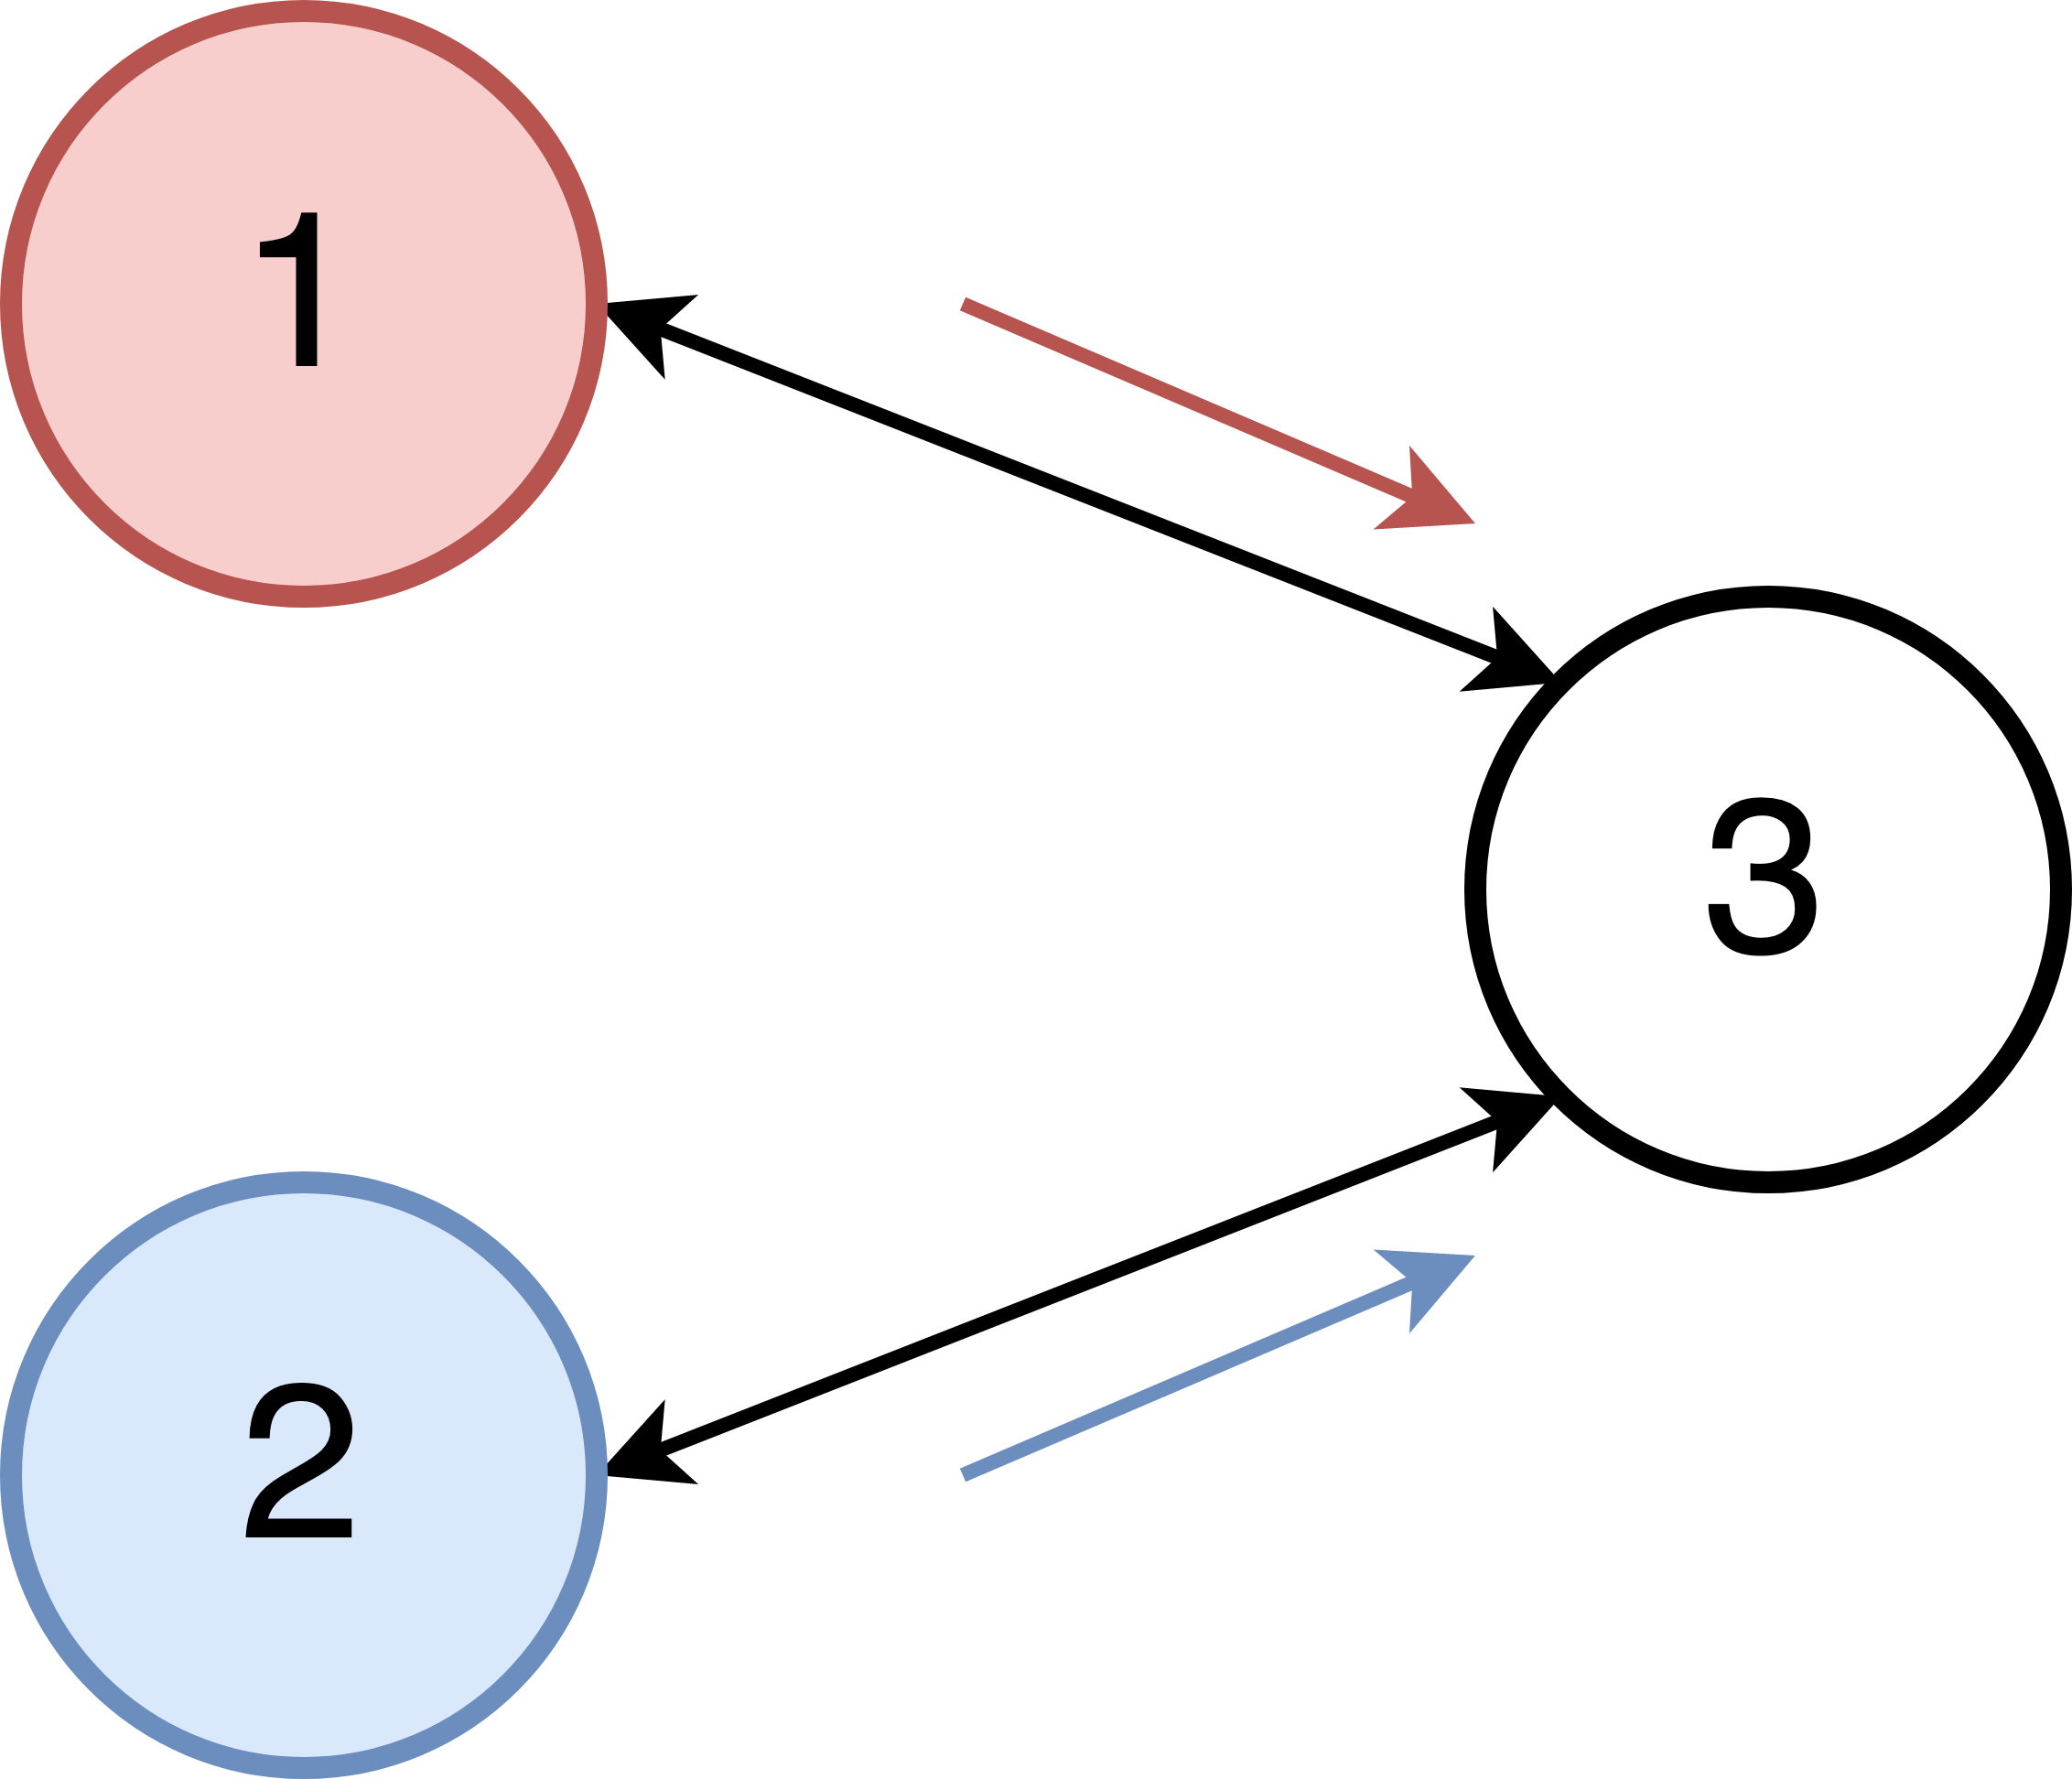
\includegraphics[width=0.65\linewidth]{vertexConflict}
    \caption{A vertex conflict occurs when two agents want to move to the same
    node at the same time.}
    \label{fig:vertexConflict}
  \end{subfigure}
  \hfill{}
  \begin{subfigure}[t]{0.3\linewidth}
    \centering
    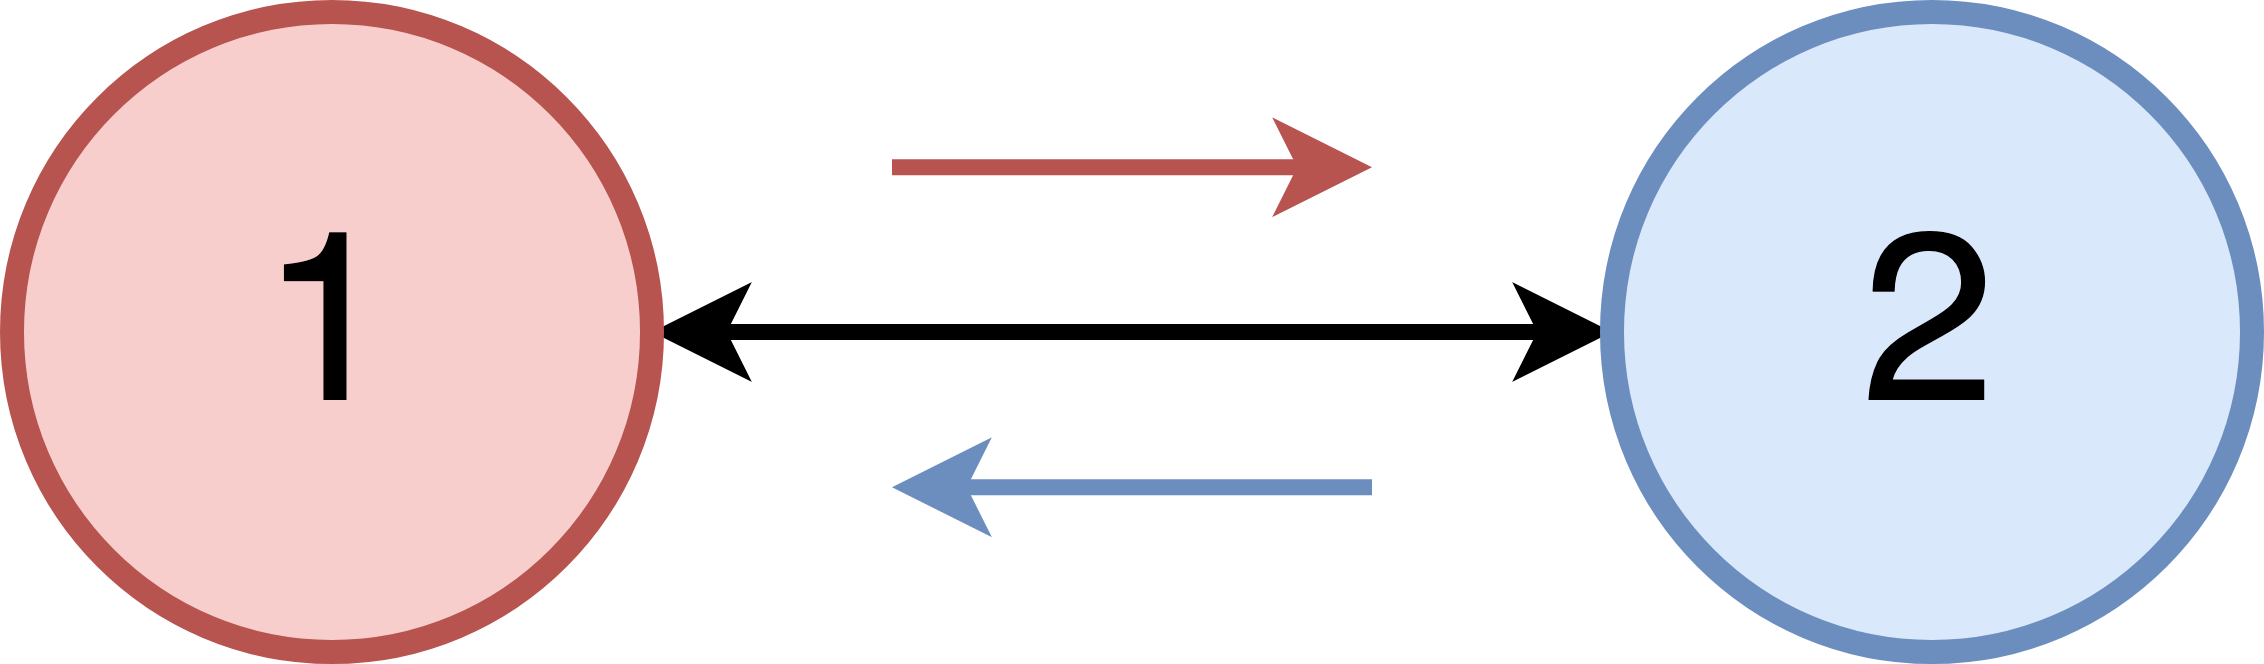
\includegraphics[width=0.65\linewidth]{swapConflict}
    \caption{A swap conflict happens when two agents want to move on the same
    edge at the same time in opposite directions.}
    \label{fig:swapConflict}
  \end{subfigure}
  \hfill{}
  \begin{subfigure}[t]{0.3\linewidth}
    \centering
    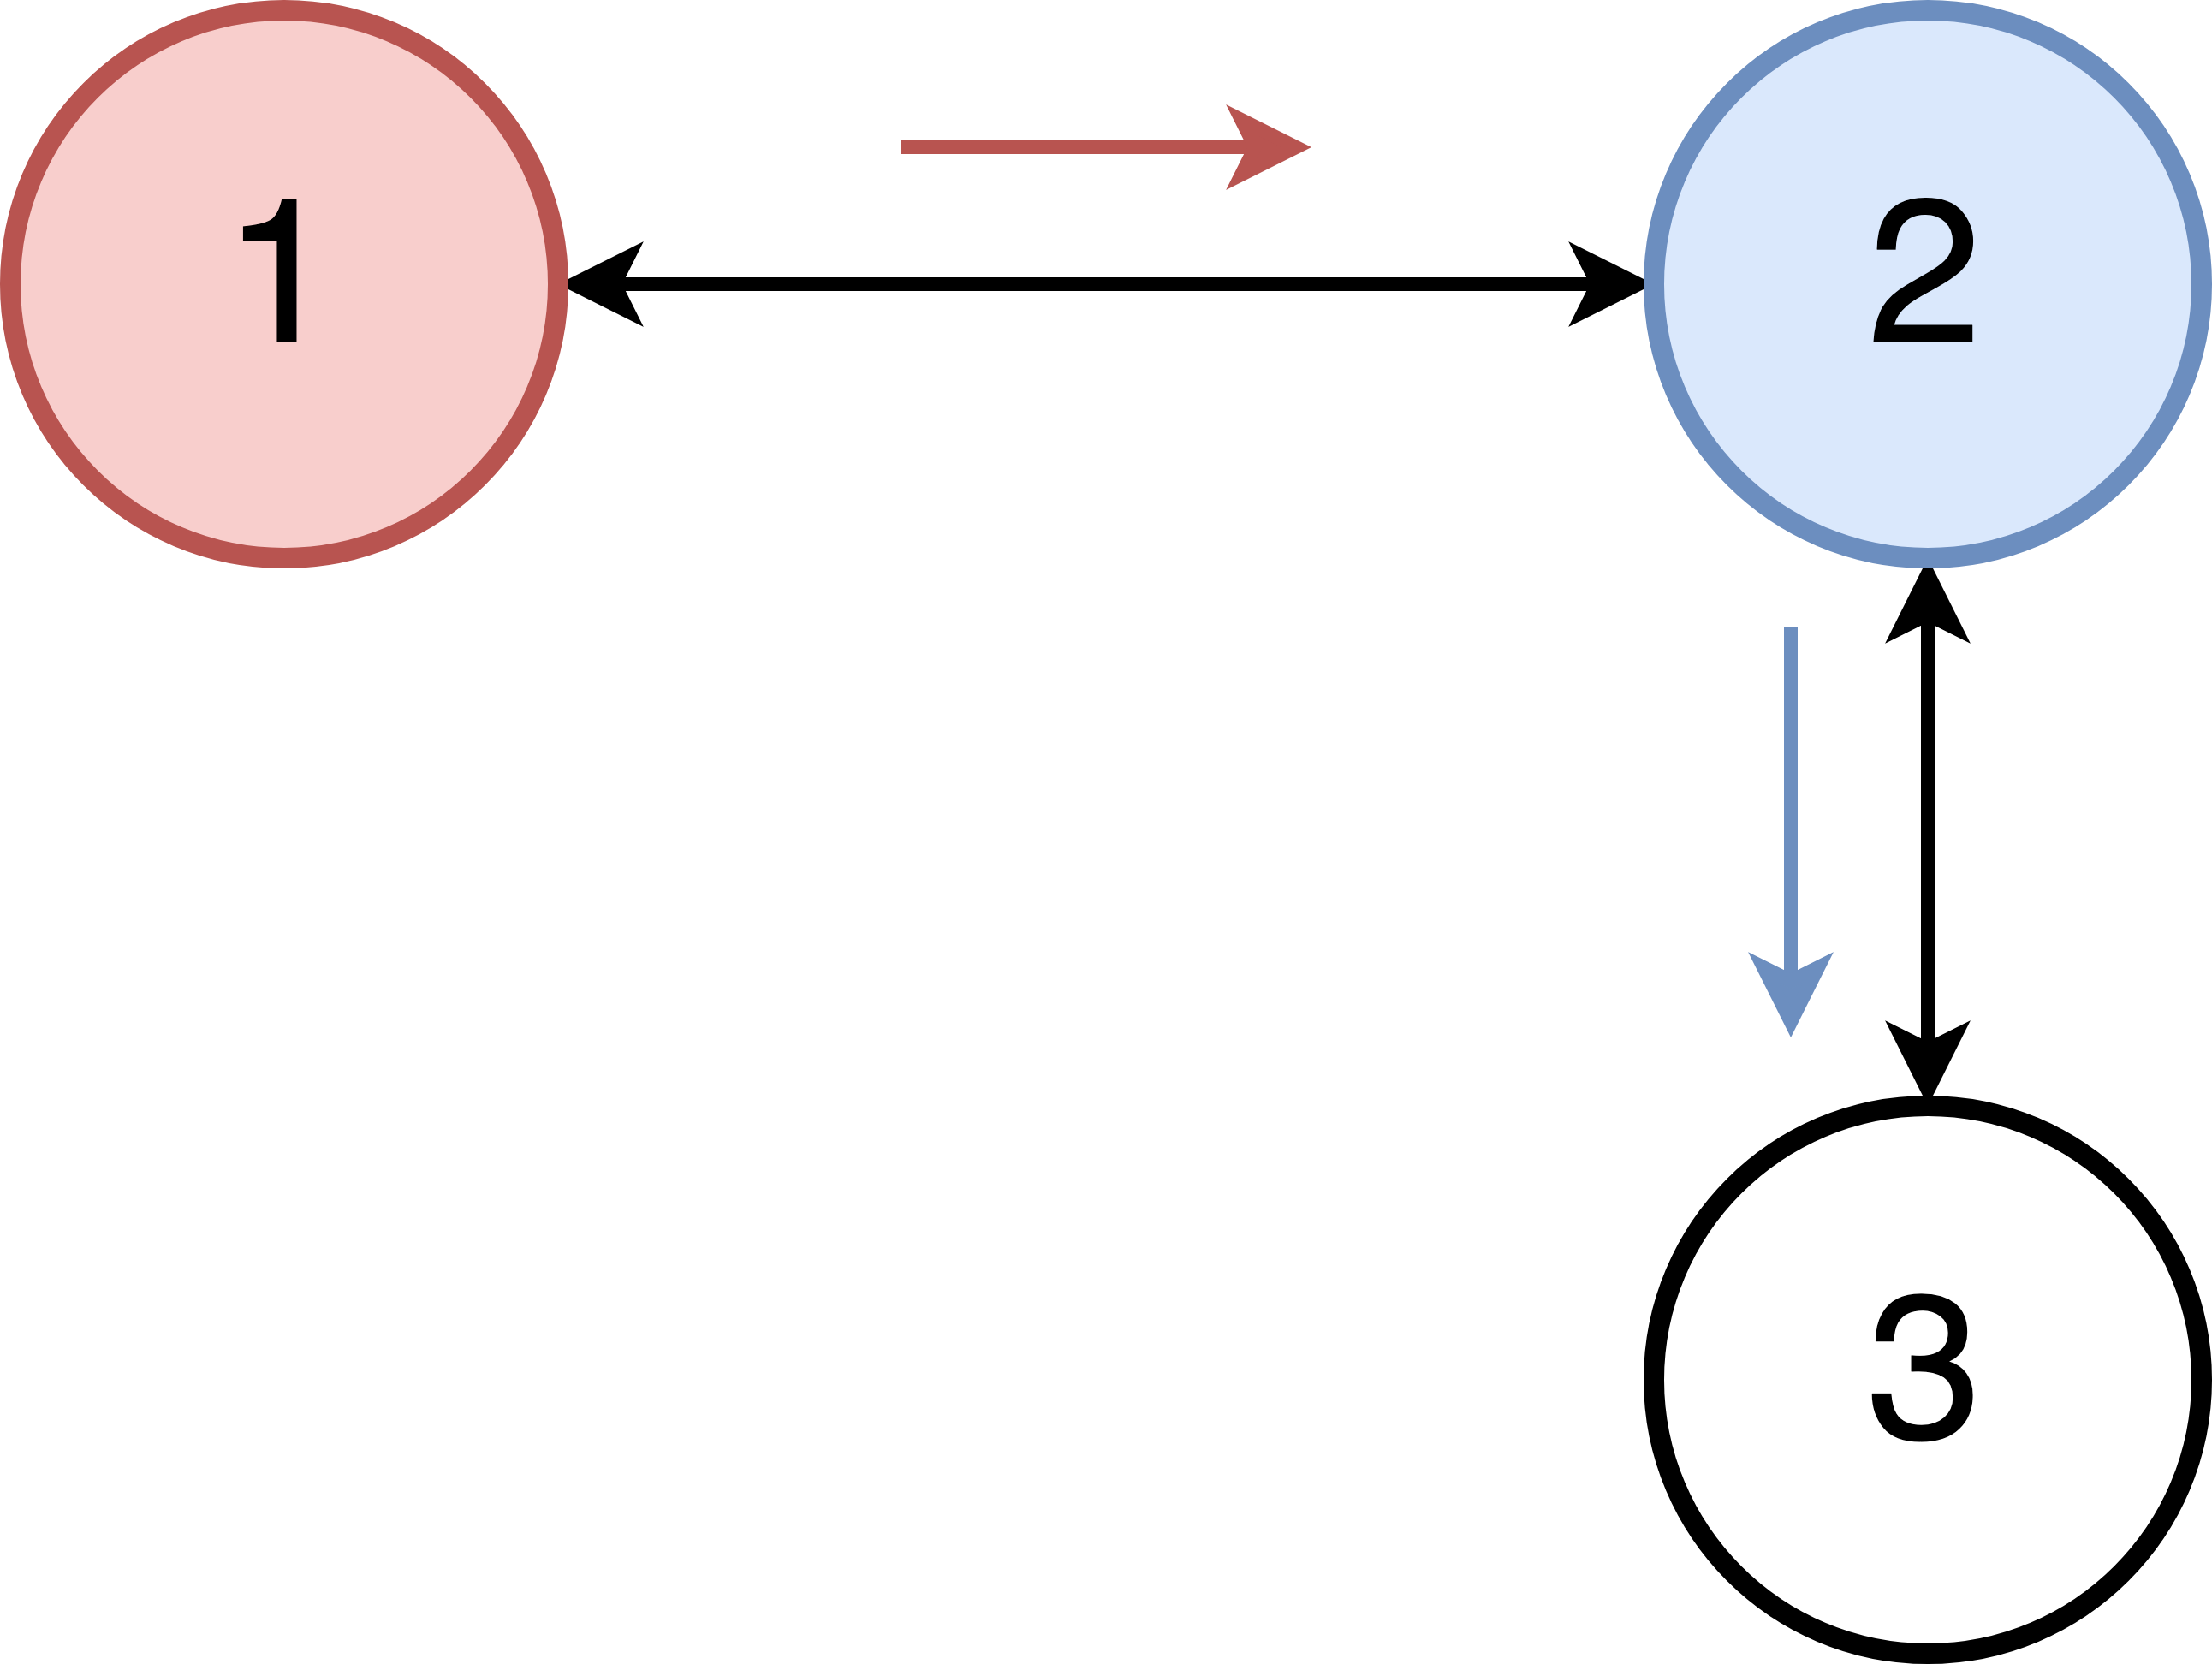
\includegraphics[width=0.65\linewidth]{followConflict}
    \caption{A follow conflict happens when an agent wants to move to a node
    that is currently occupied by another node but will be then be freed.}
    \label{fig:followConflict}
  \end{subfigure}
  \caption{The most common type of conflicts considered for the \acrs{MAPF}
  problem.}
  \label{fig:conflicts}
\end{figure} \newline
Another important aspect of the \acrs{mapf} problem is the objective function
to minimize. The reason to have a cost to minimize is due to the fact that the
problem may otherwise have different solutions as it is possible to see in
Figure~\ref{fig:mksvssic}. The classical problem considers mainly two objective
functions: the \textit{makespan} and the \textit{sum of costs}. 
\begin{figure}[t]
  \centering
  \begin{minipage}{0.38\linewidth}
    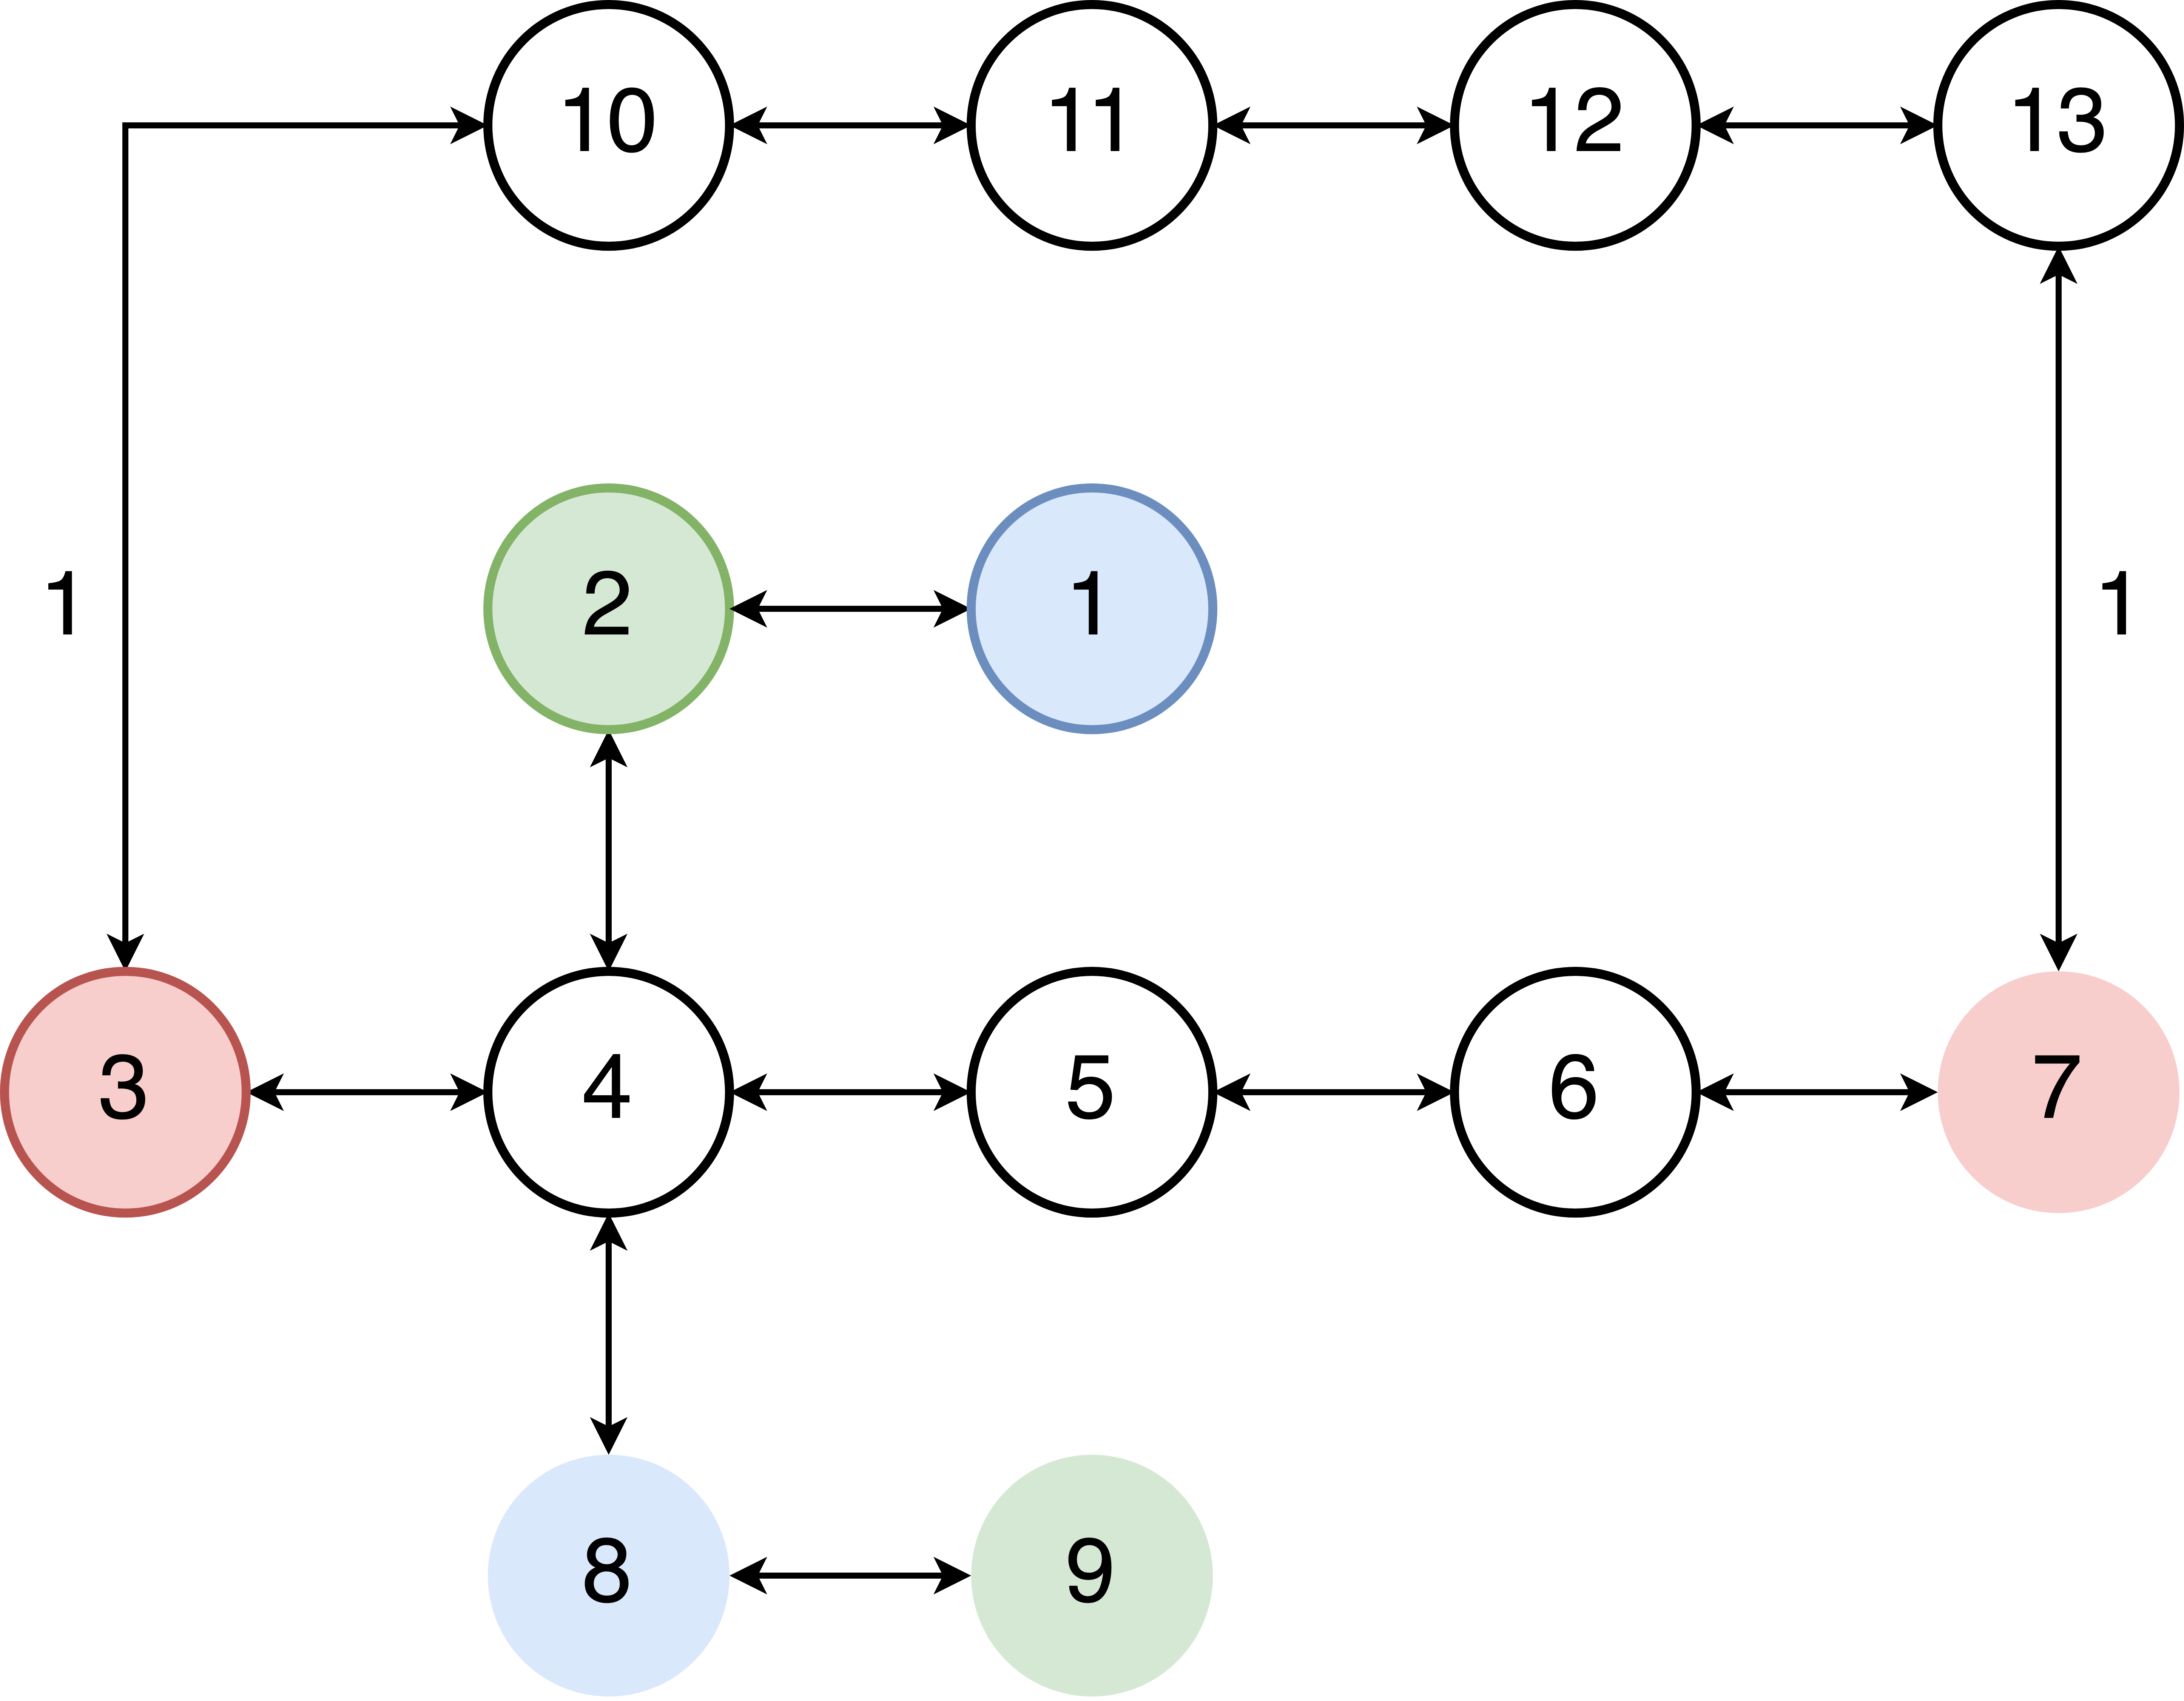
\includegraphics[width=\linewidth]{mksvssic}
  \end{minipage}
  \hfill
  \resizebox{0.58\linewidth}{!}{
    \begin{tabular}{l|c|c}
      \multicolumn{1}{c|}{$\Pi_i$} & $\sic{\Pi_i}$ & $\mks{\Pi_i}$\\
      $ \Pi_1 = 
        \begin{cases}
          \pi_1=\{3,10,11,12,13,7\}\\
          \pi_2=\{2,4,8,9\}\\
          \pi_3=\{1,2,4,8\}
        \end{cases} $ & 14 & 6 \\
        &&\\
      \hline
        &&\\
      $ \Pi_2 = 
        \begin{cases}
         \pi_1=\{3,4,5,6,7\}\\
         \pi_2=\{2,2,4,8,9\}\\
         \pi_3=\{1,1,2,4,8\}\\
       \end{cases} $ & 15 & 5 \\ 
    \end{tabular}
  }
  
  \caption{On the left a \acrs{MAPF} problem with three agents: the first agent
  in red wants to go from 3 to 7, the second agent in green wants to go from 2
  to 9 and the last agent in blue wants to go from 1 to 8. On the right a table
  summarizing the two possible solutions and showing how the solution changes
  by using one objective function instead of the other. Notice that the set of
  possible solutions is not exhaustive, although these two are the best ones 
  and hence the ones that would be chosen.}
  \label{fig:mksvssic}
\end{figure}
\newline
The makespan $\mks{\Pi}$ is a function that returns the length of the longest
path in the plan:
\begin{equation}
  \mks{\Pi}=\max\limits_{\pi_i\in\Pi}\abs{\pi_i}
  \label{eq:mks}
\end{equation}
Minimizing the makespan means finding the plan that contains the shortest path
among the possible longest paths. \newline
The sum of costs, or \acrf{SIC}, is instead the sum of the costs of all the
paths inside the plan:
\begin{equation}
  \sic{\Pi}=\Sum_{\pi\in\Pi}\abs{\pi_i}
  \label{eq:sic}
\end{equation}
%
%
\subsection{Solutions}
The classical \acrl{mapf} problem has been proved to be NP-hard, i.e., it is 
not possible to find an optimal solution in polynomial
time~\cite{lavalle,MAPFNPHARD,MAPFIntractable}. Notice that the problem is
NP-hard when finding an optimal solution, i.e., a solution that minimize the
objective function, may it be the makespan or the sum of individual costs. The
Kornhauser's algorithm~\cite{kornhauser} solves the \acrs{mapf} problem in
$O(\abs{V}^3)$, but the solution it returns it may not be the optimal one.
\newline
So an algorithm can be optimal and complete, or a combination of the two. We
say that the algorithm is \textit{optimal} if the solution it returns is the 
solution that minimizes the objective function, while we say that a solution is
suboptimal, or \textit{bounded suboptimal}, when the solution it finds 
minimized the cost within a certain degree of freedom. An algorithm is said to 
be \textit{complete} when it guarantees to return a solution.
%
\subsubsection{Kornhauser's}
The Kornhauser's algorithm is complete but not optimal. It extends the famous
15-puzzle problem which consists in having15 agents moving no a 16 4-connected
nodes graph as shown in Figure~\ref{fig:15Puzzle}, where there is only one free
node and the agents can move one step at a time to reach their final
destination.
\begin{figure}[t]
  \centering
  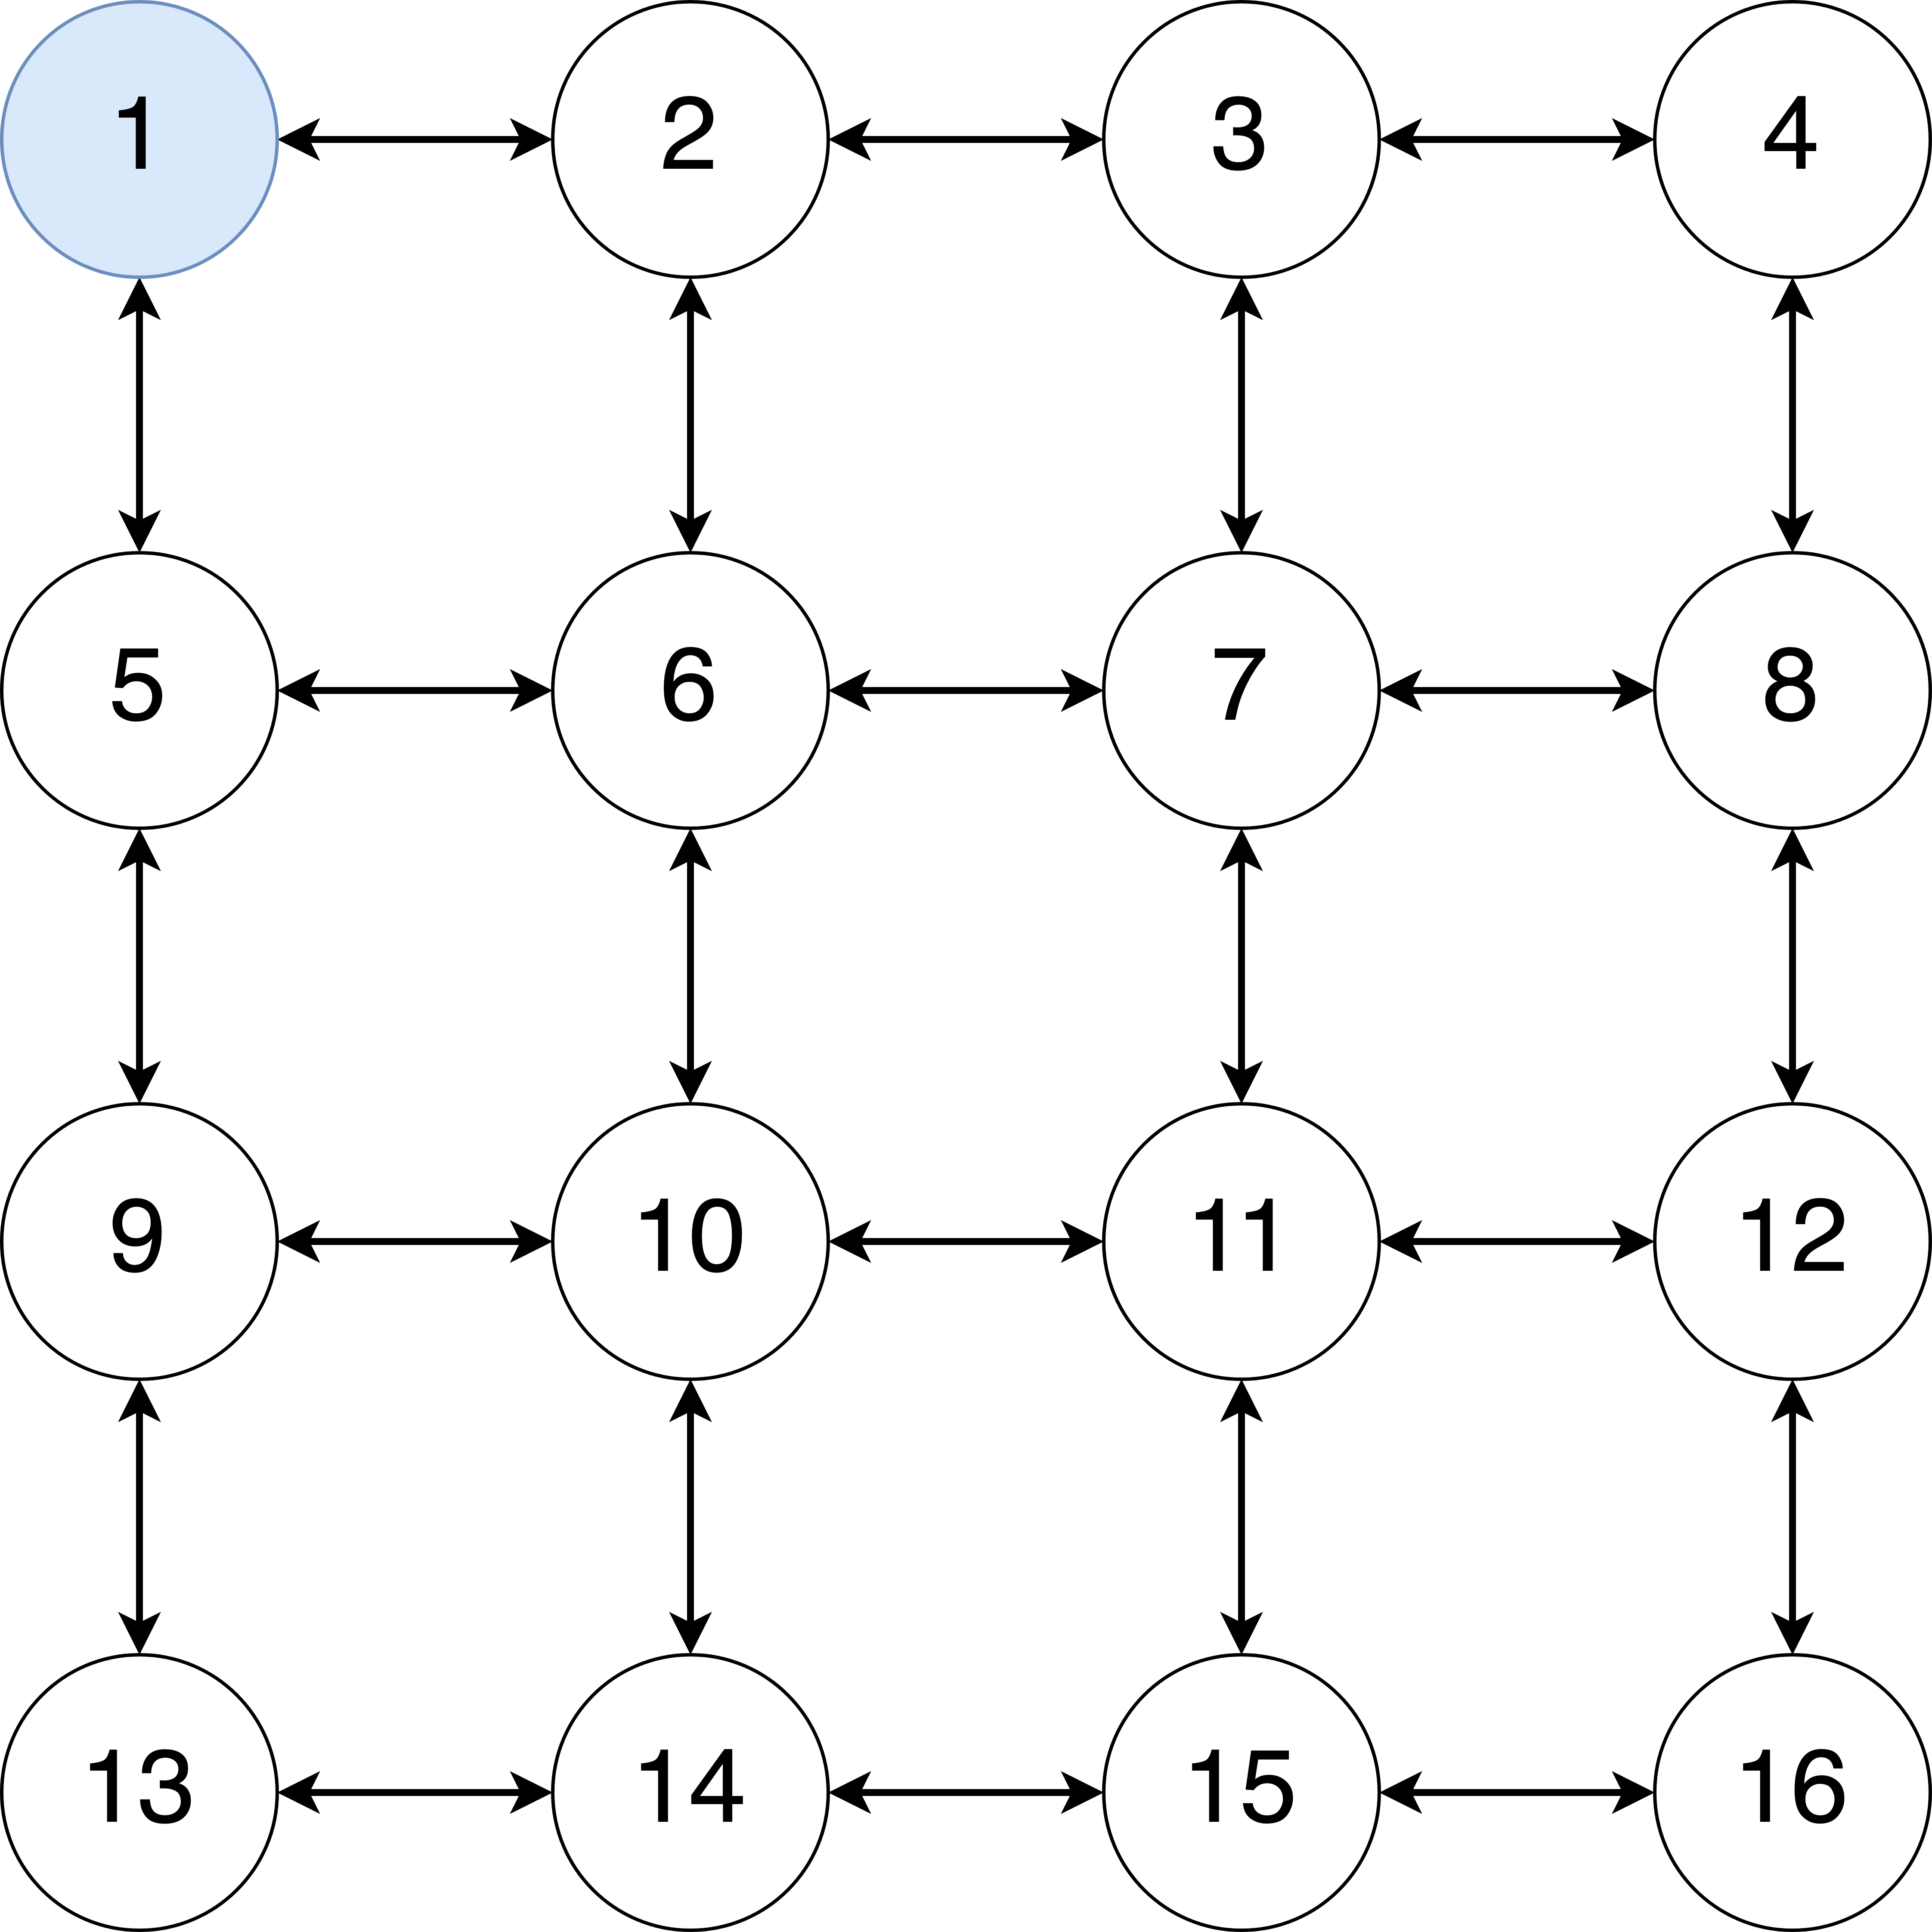
\includegraphics[width=0.35\textwidth]{15Puzzle}
  \caption{The 15 puzzle problem is a 16 node undirected graph problem in which
  there are 15 agents that need to move and only one free location
  (represented in blue.)}
  \label{fig:15Puzzle}
\end{figure}\newline
The considered generalization is the following~\cite{kornhauser}: let $G$ be a 
graph with $n$ vertices with $k<n$ agents on different vertices and let a move
be an agent shifting to a free adjacent vertex. The question the algorithm aims
to answer is whether it is possible or not to find a way to move all the agents
from one arrangement to another. The solution is obtained by decomposing the
problem in subproblems each one composed by the agents that can reach the same
set of nodes and the subgraph made of these nodes~\cite{pebble}. \newline 
The algorithm is generally considered difficult to be 
implemented~\cite{MAPF_overview} and in this work the algorithms that are
discussed are the optimal ones instead of suboptimal. 
%
\subsubsection{Extended \astar}
One could be tempted to use \astar to solve the \acrs{mapf} problem by simply
running the algorithm for each of the $k$ agents and finding the shortest path
from each node to each destination. This though proves to be really
inefficient. Indeed, by considering the search space, i.e., the number of
vertexes $\abs{V}$, and the branching factor, i.e., the average number of edges
exiting from each node, it is easy to see that the previous solution would lead
to a search space of $\abs{V}^k$ and a branching factor of
$\left(\frac{\abs{E}}{\abs{V}}\right)^k$ which are both exponential in the
number of agents and hence intractable~\cite{MAPF_overview}. \newline
Two extensions were proposed to solve the \acrs{mapf} problem~\cite{ODandID}: 
\acrf{OD} and \acrf{ID}. The first aims at reducing the exponential branching
factor while the other tries to decouple the problem of $k$ agents to smaller
problems with less agents. The two extensions can also be combined. \newline
When using \astar in \acrs{mapf} the problem is that the moves of all agents
are considered at the same time leading to an exponential branching factor. The 
idea of \acrs{OD} is to move one agent at the time, so only after $k$ moves, 
the agents will all have changed their position. The algorithm proposes a
different representation of the state space in which vertexes that represent
the positions of all agents at the same time are called \textbf{full vertexes}
and are the ones that happen every $k$ moves, while all the other vertexes are 
called \textbf{intermediate vertexes}~\cite{ODandID,MAPF_overview}. This
allows to have a branching factor of 
$O\left(k\times\frac{\abs{E}}{\abs{V}}\right)$, which is not exponential.
Moreover, it is important to notice that the heuristic used in \astar may help
in deciding whether an intermediate node is worth to be expanded speeding up
the search. \newline
\acrs{ID} is meant to reduce the main problem of $k$ agents to easier
subproblems. The idea is to start by computing the best plan for each agent as
if they were alone on the graph by using \astar. If a conflict is found, then
the two agents leading to the conflict are considered together as a meta-agent
and the best path for the two agents avoiding conflicts is computed with
\astar with \acrs{OD}. This process is iterated every time a conflict arises
and is solved by merging the new agent into the meta agent. The process stops
when there are no more conflicts~\cite{ODandID}. \newline
Notice that actually \acrs{ID} is a general framework and one could replace the
\astar with \acrs{OD} with any other \acrs{MAPF} solver. 
%
\subsection{\acrf{ICTS}}
This algorithm is actually a two-component system in which a high-level search
aims at finding the lengths of the paths for the different agents, while the 
low-level search carries out the creation of the path for the various
agents with the \textit{cost constraints} given by the high-level 
search~\cite{MAPF_overview,ICTS}. \newline
In particular, the algorithm creates a tree called \acrf{ICT} in which each 
node contains a vector of the costs $C_i$ of the individual path of each agent
$a_i$. The total cost of the node $C$ is given by the sum of the internal costs
$C=C_1+\hdots+C_k$ and all the nodes at the same level in the tree have the
same total cost. \newline
The root of the tree is initialized with the costs of the individual paths of
the agents as if they were considered in a \acrs{sapf} problem. If there are no
conflicts, then the solution is fine as it is and the algorithm stops. If 
instead a conflict was found, then $k$ new nodes are going to be created, one 
for each agent: the $i$-th node is composed of the solution of the parent, with
the only change that the cost solution for the $i$-th agent is one more than
before. The idea is the following: if with a given solution it was not possible
to find a solution without conflicts, then it may be possible to find a
solution by increasing the path of an agent by one. The algorithm continues 
until a solution is found. The \acrs{ICT} nodes not containing conflicts are 
called \textit{goal nodes}. \newline
The low-level search is instead the part of the algorithm that has to find a
path for the $i$-th agent of cost $C_i$ and such that it reaches its final
destination. There may be different implementations for this part of the
algorithm: the most trivial would be to start from the initial node and
enumerate all the possible path of length $C_i$ and check which are reaching
the final node. This though may become very expensive as the number of possible
paths of cost $C_i$ may be exponential. The solution proposed~\cite{ICTS} uses
an \acrf{MDD}~\cite{MDD} which are a generalization of the binary decision
diagrams in the sense that they allow for more than two choices for every node.
Basically, the \acrs{MDD} has a single source node which corresponds to the
starting node of the agent. Then, it keeps track of all the neighbors of the
source node adding them only if the path going through them can lead to the
final node with cost $C_i$. This implies also that the \acrs{MDD} has a single
sink and that it is the final goal of the agent. \newline
The problem is then how to choose which path is best to return to the
high-level search since a path may produce more conflicts than another leading
to a bigger and sub-optimal \acrs{ICT}. This is done by doing the
cross-product, i.e., merging, the different \acrss{MDD} and removing those
branches that contains conflicts. 
Notice two things: given the structures of the \acrs{ICT} and of the 
cross-product of the \acrss{MDD}, the optimization problem can be reduced to a
satisfaction problem: the first \acrs{ICT} node that satisfy the constraint of
not having any conflict is also going to be optimal, and the same is true for
the paths found in the combination of the \acrss{MDD}.
\begin{figure}[tb]
  \centering
  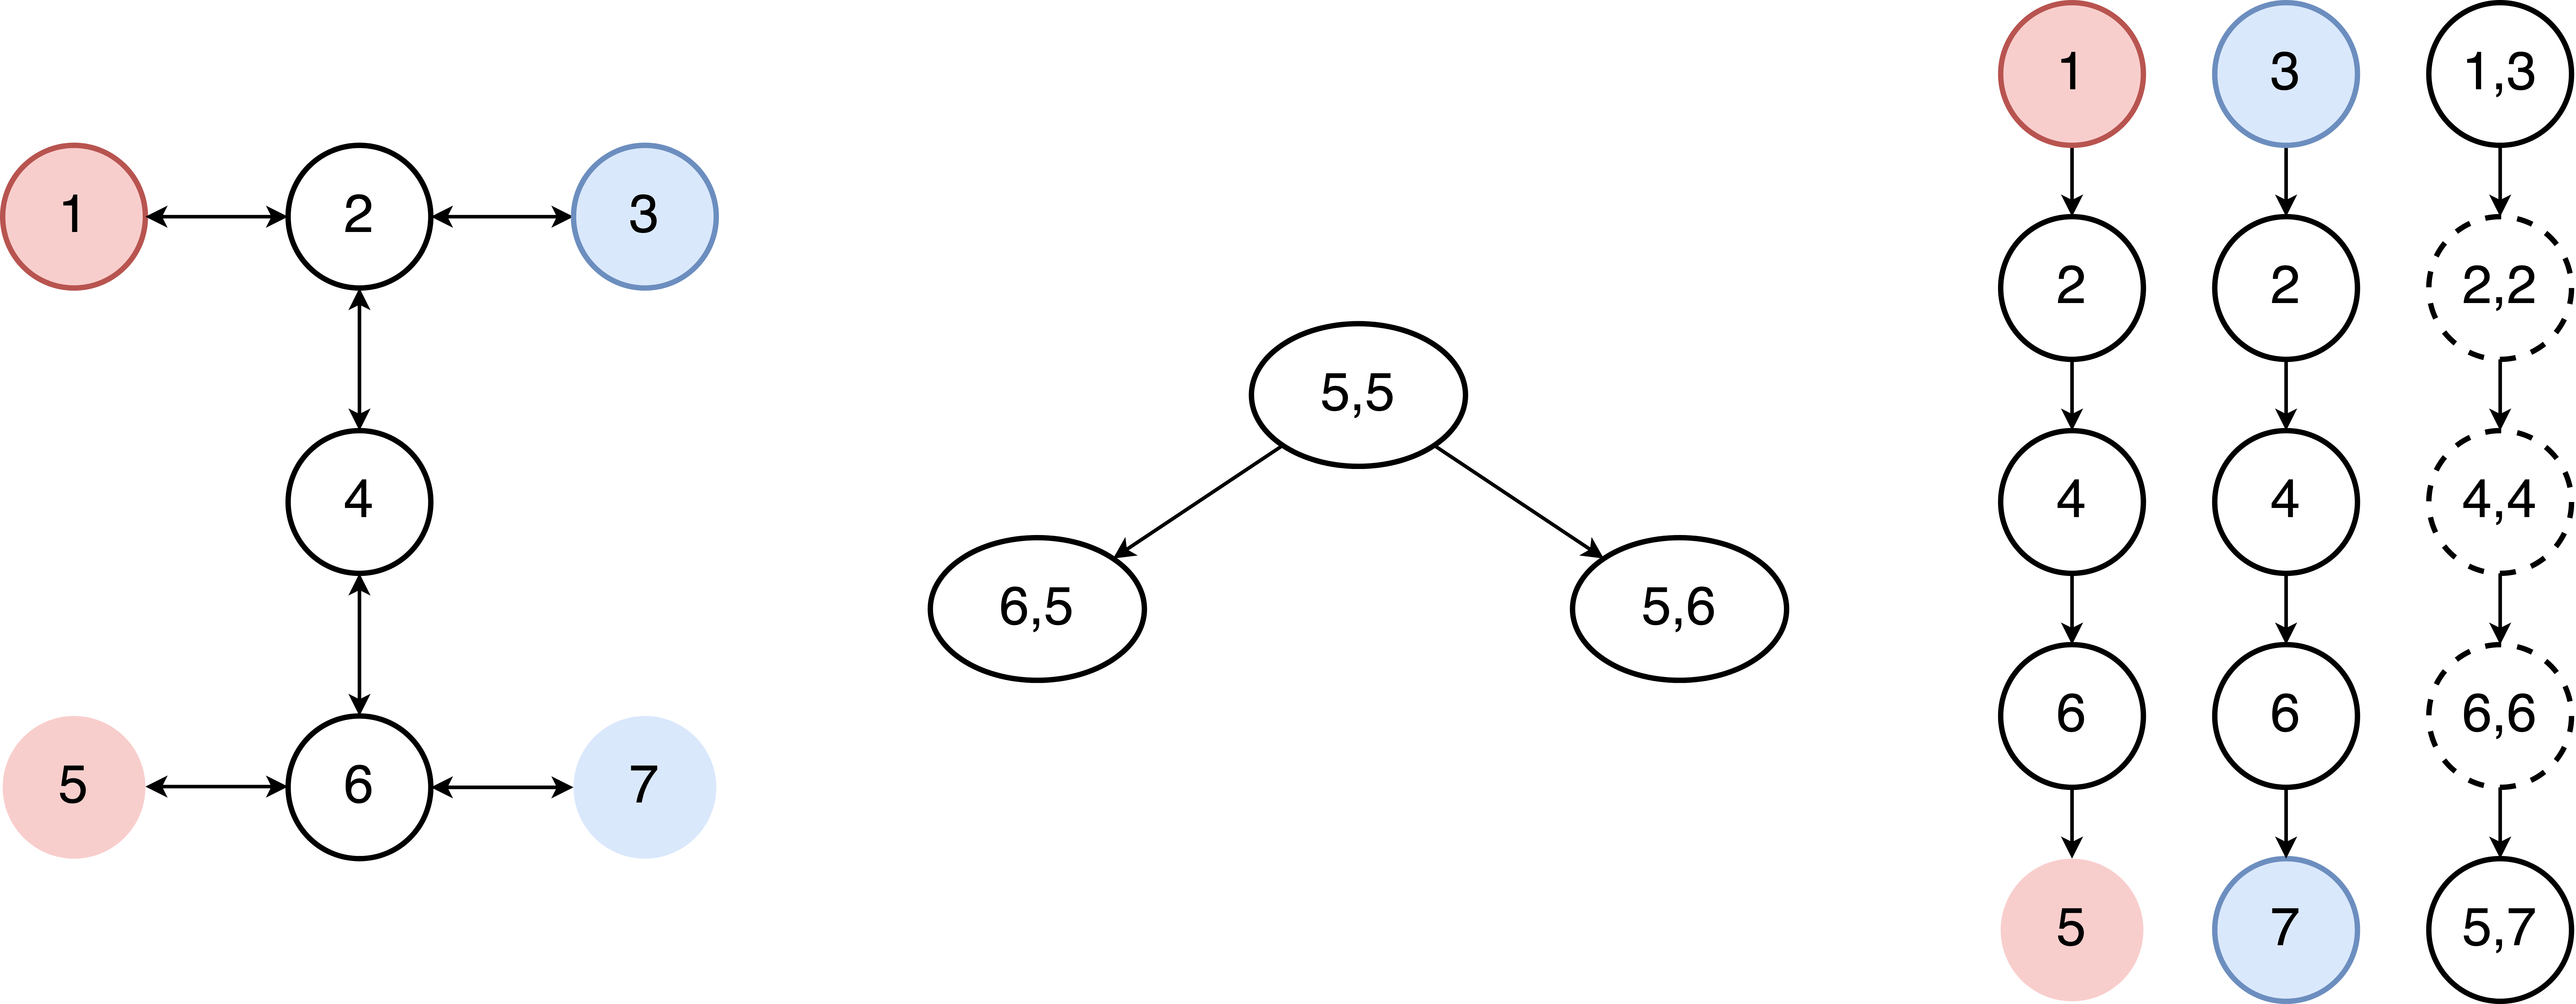
\includegraphics[width=0.8\textwidth]{ICTS}
  \caption{On the left a \acrs{MAPF} problem with two agents: one moving from 1
  to 5 and the other moving from 3 to 7. In the middle, the \acrs{ICT} that
  comes from solving the problem by using \acrs{ICTS}: the algorithm starts
  with the lengths of the paths as if solving a \acrs{sapf} problem. By finding
  a conflict as depicted in the \acrss{MDD} on the right, it creates two nodes
  and tries to find a combination of paths solving the problem with those
  costs. Finally, on the right, the two \acrss{MDD} for the two agents with
  cost $5$ and the combination of the \acrss{MDD} showing the conflicts with
  dotted lines.}
  \label{fig:ICTS}
\end{figure}
%
\subsection{\acrf{CBS}}
\label{ssec:cbs}
Similarly to \acrs{ICTS}, it uses two distinct search processes, a high-level 
and a low-level one, and a tree to solve the \acrs{MAPF} problem. \newline
The \acrs{CBS} tree is called \acrf{CT} and is composed of nodes tracking three
elements: 
\begin{itemize}
  \item The joint plan; 
  \item The cost of the joint plan;
  \item A set of \textit{constraints} associated with the joint plan.
\end{itemize}
The idea is that whenever a joint plan contains a conflict, it is resolved by
creating two new nodes with different constraints, which are limitations of an
agent movement. In particular, the original \acrs{CBS}~\cite{CBS} defines
constraint as a negative restriction tuple $(a_i, n, t)$, meaning that the
agent $a_i$ is not allowed to be on node $n$ at time $t$. \newline
The protocol works in the following way: the root is built by considering the
paths of the agents as in a \acrf{sapf} problem. Then, the high-level search
checks for possible conflicts. Let $\pi_i$ and $\pi_j$ be the plans for agents
$a_i$ and $a_j$ respectively, and suppose that they have a vertex conflict at
time $t$ on node $n$. Then, the high-level search creates two new \acrs{CT}
nodes from the parent, one in which agent $a_i$ \textit{cannot} be on node $n$
at time $t$, and the other \acrs{CT} node in which agent $a_j$ \textit{cannot}
be on node $n$ at time $t$. \newline
An improvement to \acrs{CBS}~\cite{ICBS} suggests that using two positive
constraints and a negative one may produce better results since the set of
paths that complies with the constraints is disjoint~\cite{MAPF_overview}. This
means that, instead of having two children from a node, the high-level search
creates three children, one in which agent $a_i$ must be on node $n$ at time
$t$, one in which agent $a_j$ must be on node $n$ at time $t$ and one in which
neither of them is allowed to be on node $n$ at time $t$. \newline
The process of expanding nodes, i.e., creating new children, stops when there
are no more conflicts to be solved. \newline
Whenever a new node is added, the low-level search is called to find a solution
to the problem with the new added constraints. If a feasible solution can be
found, then the node is added to the set of nodes to be further explored. To
pick the next node to examine, \acrs{CBS} uses the cost function of the joint
plan. \newline
Finally, as it regards the low-level search, it can be any \acrs{SAPF}
algorithm, although it needs to be properly modified to support the presence of
constraints. 
%
\subsection{\acrf{CP} and \acrf{MILP}}
Constraint programming is an alternative approach to the imperative paradigm,
which is mainly used when coding~\cite{CP}. \acrs{MILP} is a mathematical
modeling paradigm in which the decision variables are subject to some
inequalities. These types of programming are usually divided into two parts: a
first one called modelling that addresses the shaping of the aspects of the
problem introducing variables over specific domains and constraints over such
variables. A second part instead aims at choosing how to solve the
representation of the problem that was modelled. There are various types of
solver, for example, one could use a \acrs{CP} solver or model the problem so
that it can be solved with \acrf{SAT} or \acrf{MIP} solvers. \newline
If the constraints are well-formed, i.e., they correctly cover the variables
and their domains, than \acrl{cp} is both optimal and correct. A brief
description of the constraint used in~\cite{picat1} to solve the \acrs{MAPF}
problem is now carried out, a deeper and more precise one will be performed
later on. The main constraints that are needed are the
following~\cite{MAPF_overview}:
\begin{itemize}
  \item Agents occupy only one vertex in each time step: this is to ensure that
    we are solving the classical \acrs{MAPF}, whereas a \acrs{MAPF} problem for
    large agents takes into consideration the fact that each agent may occupy
    more than 1 vertex at a time;
  \item A node can be occupied by only one agent in each time step: it
    guarantees that there are no vertex conflict;
  \item Agents are positioned on their initial position at the first time step,
    and must be on their arrival position at the last time step;
  \item Agents move along edges towards neighbors of the node on which they 
    are: this is to ensure the validity of the solution since an agent cannot
    jump from one node to another. 
\end{itemize}
Once the constraints are fixed, the model can be solved with a solver, which
tries to look at all the possible combinations without infringing any
constraint. 
%
%
\subsection{\acrs{MAPF} Variations}
Below, a brief description of some \acrs{MAPF} variations is carried out. The
list is not exhaustive as it introduces only those variations from which some
key aspects have been taken into consideration to model the problem this work
focuses on. 
%
\subsubsection{\acrf{MAPD}}
The \acrf{mapd} is a problem that strictly relates to the \acrl{mapf} one. 
While \MAPF aims at finding a feasible path for all the agents in the system 
from a starting position to a desired destination, the \acrs{MAPD} problem 
introduces the option for all the agent to have to meet an intermediate 
position. Indeed, in an industrial environment, robots usually need to complete
a task by starting from an initial position then to move to an intermediate one 
called "pickup" location and finally to reach their delivery location. \newline
This introduces a remarkable difference from \acrs{MAPF}, which can be seen as
a one-shot version of the problem~\cite{onlineMAPD}.\newline
Similarly to the \MAPF, also the \acrs{MAPD} problem consists of $m$ agents
$\mathcal{A}=\{a_1,a_2,\hdots,a_m\}$ and an undirected connected graph 
$G=(V,E)$, where $V$ is the set of the vertices, i.e., the locations, and $E$
is the set of the edges, i.e., the connections between locations that the
agents can travel through. Let an agent $a_i$ start from a location $l_i(0)$,
then at each timestamp $t$, the agent either stays in the same position
$l_i(t+1)=l_i(t)$ or it moves to a neighboring node $(l_i(t), l_i(t+1))\in E$.
Moreover, as for the \MAPF problem, \textit{vertex} and \textit{swap} conflicts
should be avoided, that is two agents $a_i, a_j$ cannot be on the same node at 
the same time $l_i(t)\neq l_j(t)$ and they cannot move on the same edge at the
same time in opposite directions $l_i(t+1)\neq l_j(t) \wedge l_j(t+1)\neq
l_i(t)$, respectively. \newline
The part that mainly differs from the \MAPF problem is the fact that the agents
need to complete \textit{tasks}. A task $\tau_j$ can be defined as the tuple
$(s_j,g_j)$, where $s_j\in V$ is the pickup location and $g_j\in V$ is the 
destination to be reached. An agent is called \textit{free} at a certain moment
$t$ if it is not executing any task, otherwise it is called 
\textit{occupied}~\cite{onlineMAPD}. Notice that the agent is bound to a given
task from the moment it reaches the pickup location, i.e., if an agent $a_i$ is
associated with a task $\tau=(s, g)$, but has not reached $s$ yet, then another
agent $a_j$ may take over, e.g., when $a_j$ is closer to $s$ than $a_i$ is.
Consider a task set $\mathcal{T}$ in which the system inserts all the 
unexecuted tasks, then the goal of the problem is to execute all the tasks 
$\tau\in\mathcal{T}$.
\begin{figure}[tpb]
  \centering
  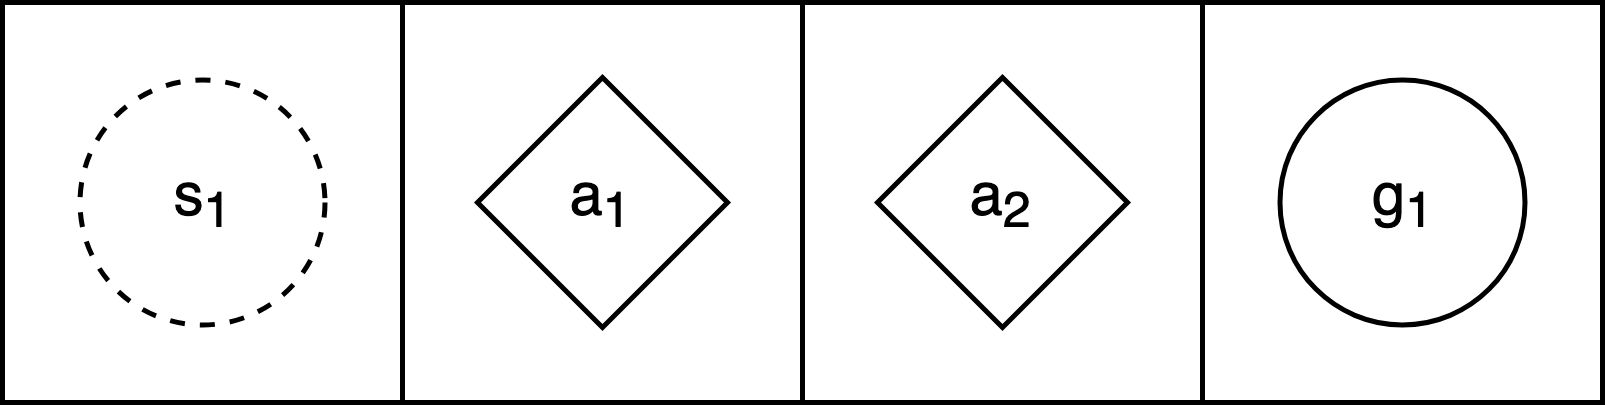
\includegraphics[width=0.4\textwidth]{onlineMAPD1}
  \caption{The figure shows a \acrs{MAPD} instance which is not solvable. The
  example shows an environment with two agents, $a_1, a_2$ and a task set
  $\mathcal{T}=\{\tau_1=(s_1,g_1)\}$. The instance is not solvable because 
  $a_2$ cannot move to $s_1$ without a vertex conflict and neither can $a_1$ 
  reach $g_1$ without a vertex conflict. }
  \label{fig:onlineMAPD1}
\end{figure}
\newline
As presented up until now, the problem is as wide as possible. In this case,
there are instances that are not solvable, for example the one shown in
Figure~\ref{fig:onlineMAPD1}. One possibility is to consider only well-formed,
or \textit{valid}, \acrs{MAPD} instances~\cite{wellFormedMAPD}. The idea is 
that agents can rest only on locations called \textit{non-task endpoints}, that 
is locations from where no other agent is blocked. \newline
One final distinction is done between \textit{offline} and \textit{online}
\acrs{MAPD} problems. The former assumes that all the tasks are known \textit{a 
priori} and no other task will be added to the task set during the execution of
the agents. Instead, the latter means that new tasks may continue to arrive and
that no information regarding the number of the tasks, nor their structure is
known \textit{a priori}. 
%
\subsubsection{Online MAPD Algorithms}
The state-of-the-art algorithms for solving the offline \acrs{MAPD} problem are
discussed in~\cite{onlineMAPD}, in which the authors presents two decoupled 
algorithms (\acrf{TP} and \acrf{TPTS}) and a centralized one called
\texttt{CENTRAL}. \newline
\acrs{TP} and \acrs{TPTS} use a token, i.e., a synchronized shared block of
memory, which contains the agents current paths, the task set and the agents
assignments. A central system is in charge to pass the token to the agents
which do the computations on their own. Indeed, the first step of the
algorithms consists in the system initializing the token with trivial paths in
which the agents stay on their initial locations. Then, whenever an agent 
reaches the end of the path as described in the token, it requests the token
from the system and chooses a new task to execute making sure that the pickup
and delivery locations of the new task do not produce a conflict with the paths
of the other agents. Two possibility may arise:
\begin{itemize}
  \item Such a task exists, then the agent chooses the task removing it from
    the task set and updates its path in the token trying to find a path that
    minimizes the cost while still avoiding collisions; or
  \item there is no such task, then it checks all the tasks in the task set to
    make sure that its current position is not a delivery location. If it
    is not, then the token is updated with a stay path, otherwise an auxiliary
    function is called, which will move the agent to a chosen endpoint without
    creating conflicts. 
\end{itemize}
\acrs{TPTS} adds to \acrs{TP} the possibility of swapping a task if the agent
assigned to it has not arrived to the pickup location yet. To do this, the task
set does not contain only unassigned tasks, but also unexecuted ones. If a task
$\tau$ is assigned to an agent $a_i$, but it is not yet been executed, then a
second agent $a_j$ can swap in and assign itself the task. For example, this
may be done when the latter agent can reach the pickup location in fewer steps 
than the former. When a swap happens, $a_j$ sends the token to $a_i$ which can
check if it can assign a new task to itself. 
%
\subsubsection{Non-unitary edges}
As said in Section~\ref{sec:MAPF}, classical \acrs{mapf} considers an
undirected graph with edges that have unitary cost, that is, the cost of an
action is always one when computing the objective function, independently by
the fact that the agent moved over an edge or stayed on a node. This introduces
a constraint regarding the possible movements of the agents. Indeed, the main
problem with having edges with different costs is the fact that agents may
conclude their actions in different times causing only a portion of the action
to overlap. Walker et al. proposed a solution showing great results when
applied to the \acrs{ICTS} algorithm proposing two new variations called
$\varepsilon-$\acrs{ICTS} and $\omega-$\acrs{ICTS}~\cite{EICTS}. \newline
Both algorithms consider an agent either staying on the vertex or moving from
one vertex to another traversing an edge at constant speed. A collision is
defined as the condition for which one or more agents overlap at the same
instant of time. The collision check is done by considering only agents with
partial time overlaps and then by running a continuous-time conflict detection
algorithm for moving agents~\cite{collision_detection}. \newline
Then, the multi-value decision diagram of the low-level search of \acrs{ICTS}
needs to be changed to account for different costs and especially for the fact
that non-unitary costs may lead to have multiple sink. For example, looking at
Figure~\ref{fig:eICTS}, it is possible to notice that a 4-connected
grid\footnote{A 4-connected grid is a grid where the nodes are connected only
upwards, leftward, rightward and downwards} generates only one sink for the
goal node at a given time, whereas if the graph was fully connected, then the
possible sink in a given interval could be more than one. This problem depends
on the value set to discretize the increment of time. Indeed, if the value is
small, the possibility of finding multiple sinks in the graph in an interval of
time is smaller, but at the same time the depth of the graph will increase. On
the contrary, a larger value of the increment may lead to a higher probability
of finding multiple sinks, but to a smaller graph. \newline
Some changes had to be made also to the high-level search. In the original
protocol, the nodes would keep track of only the cost of the paths for each
agent. In the extended versions, each node keeps track of a lower and an upper
bound for each agent, other than the path. The low-level will not return the
existence of a solution, but it will return the cost in the interval between
the lower bound and the upper bound. The final solution is then obtained in a
best-first manner. \newline
The proposed algorithms $\varepsilon$-\acrs{ICTS} and $\omega$-\acrs{ICTS}
provide the following improvements:
\begin{itemize}
  \item $\varepsilon$-\acrs{ICTS}: instead of finding the optimal solution, the
    low-level search exits on the first feasible solution. This allows the
    algorithm to save time and space in the high-level, but at the cost of 
    optimality.
  \item $\omega$-\acrs{ICTS}: the value of the increment is obtained
    dynamically by computing a ratio between the weighted cost of the previous
    iteration and the number of agents.
\end{itemize}
\begin{figure}[htpb]
  \centering
  \begin{subfigure}[t]{0.49\linewidth}
    \centering
    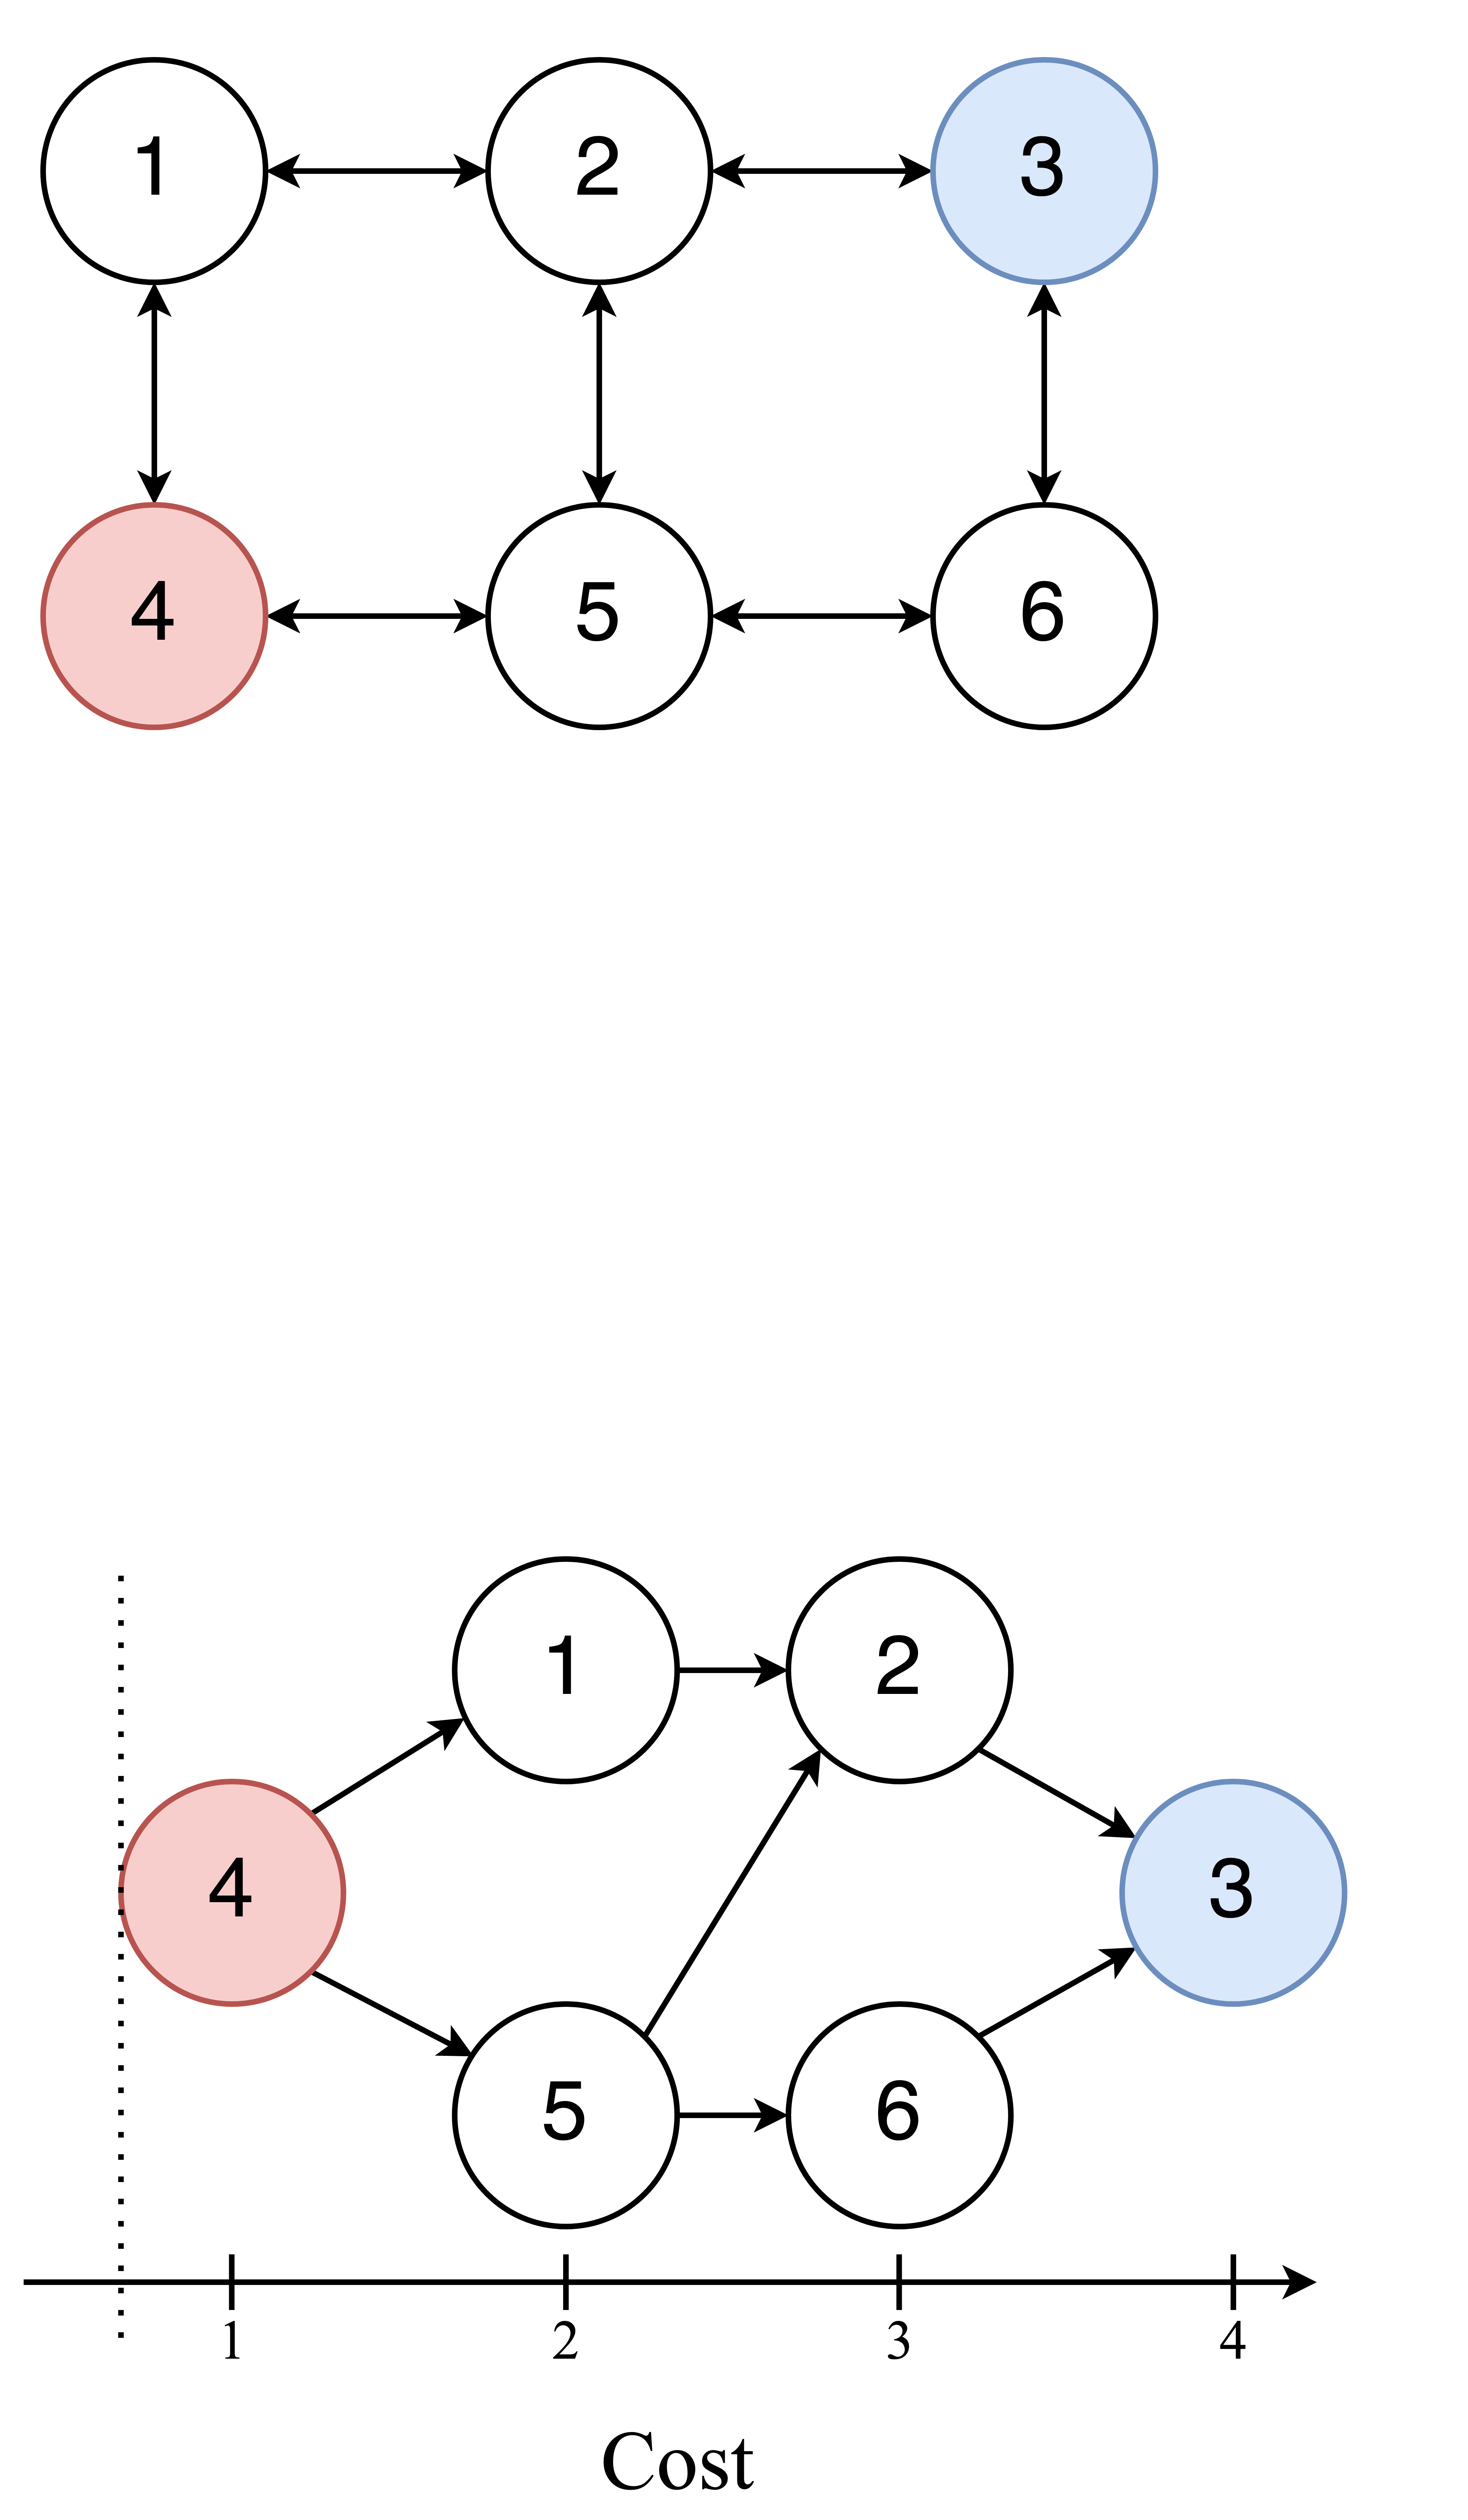
\includegraphics[width=0.7\linewidth]{ICTSNonUnit1}
    \caption{On the left, a standard \acrs{MAPF} problem where each edge has
      weight one.} 
  \end{subfigure}
  \hfill
  \begin{subfigure}[t]{0.49\linewidth}
    \centering
    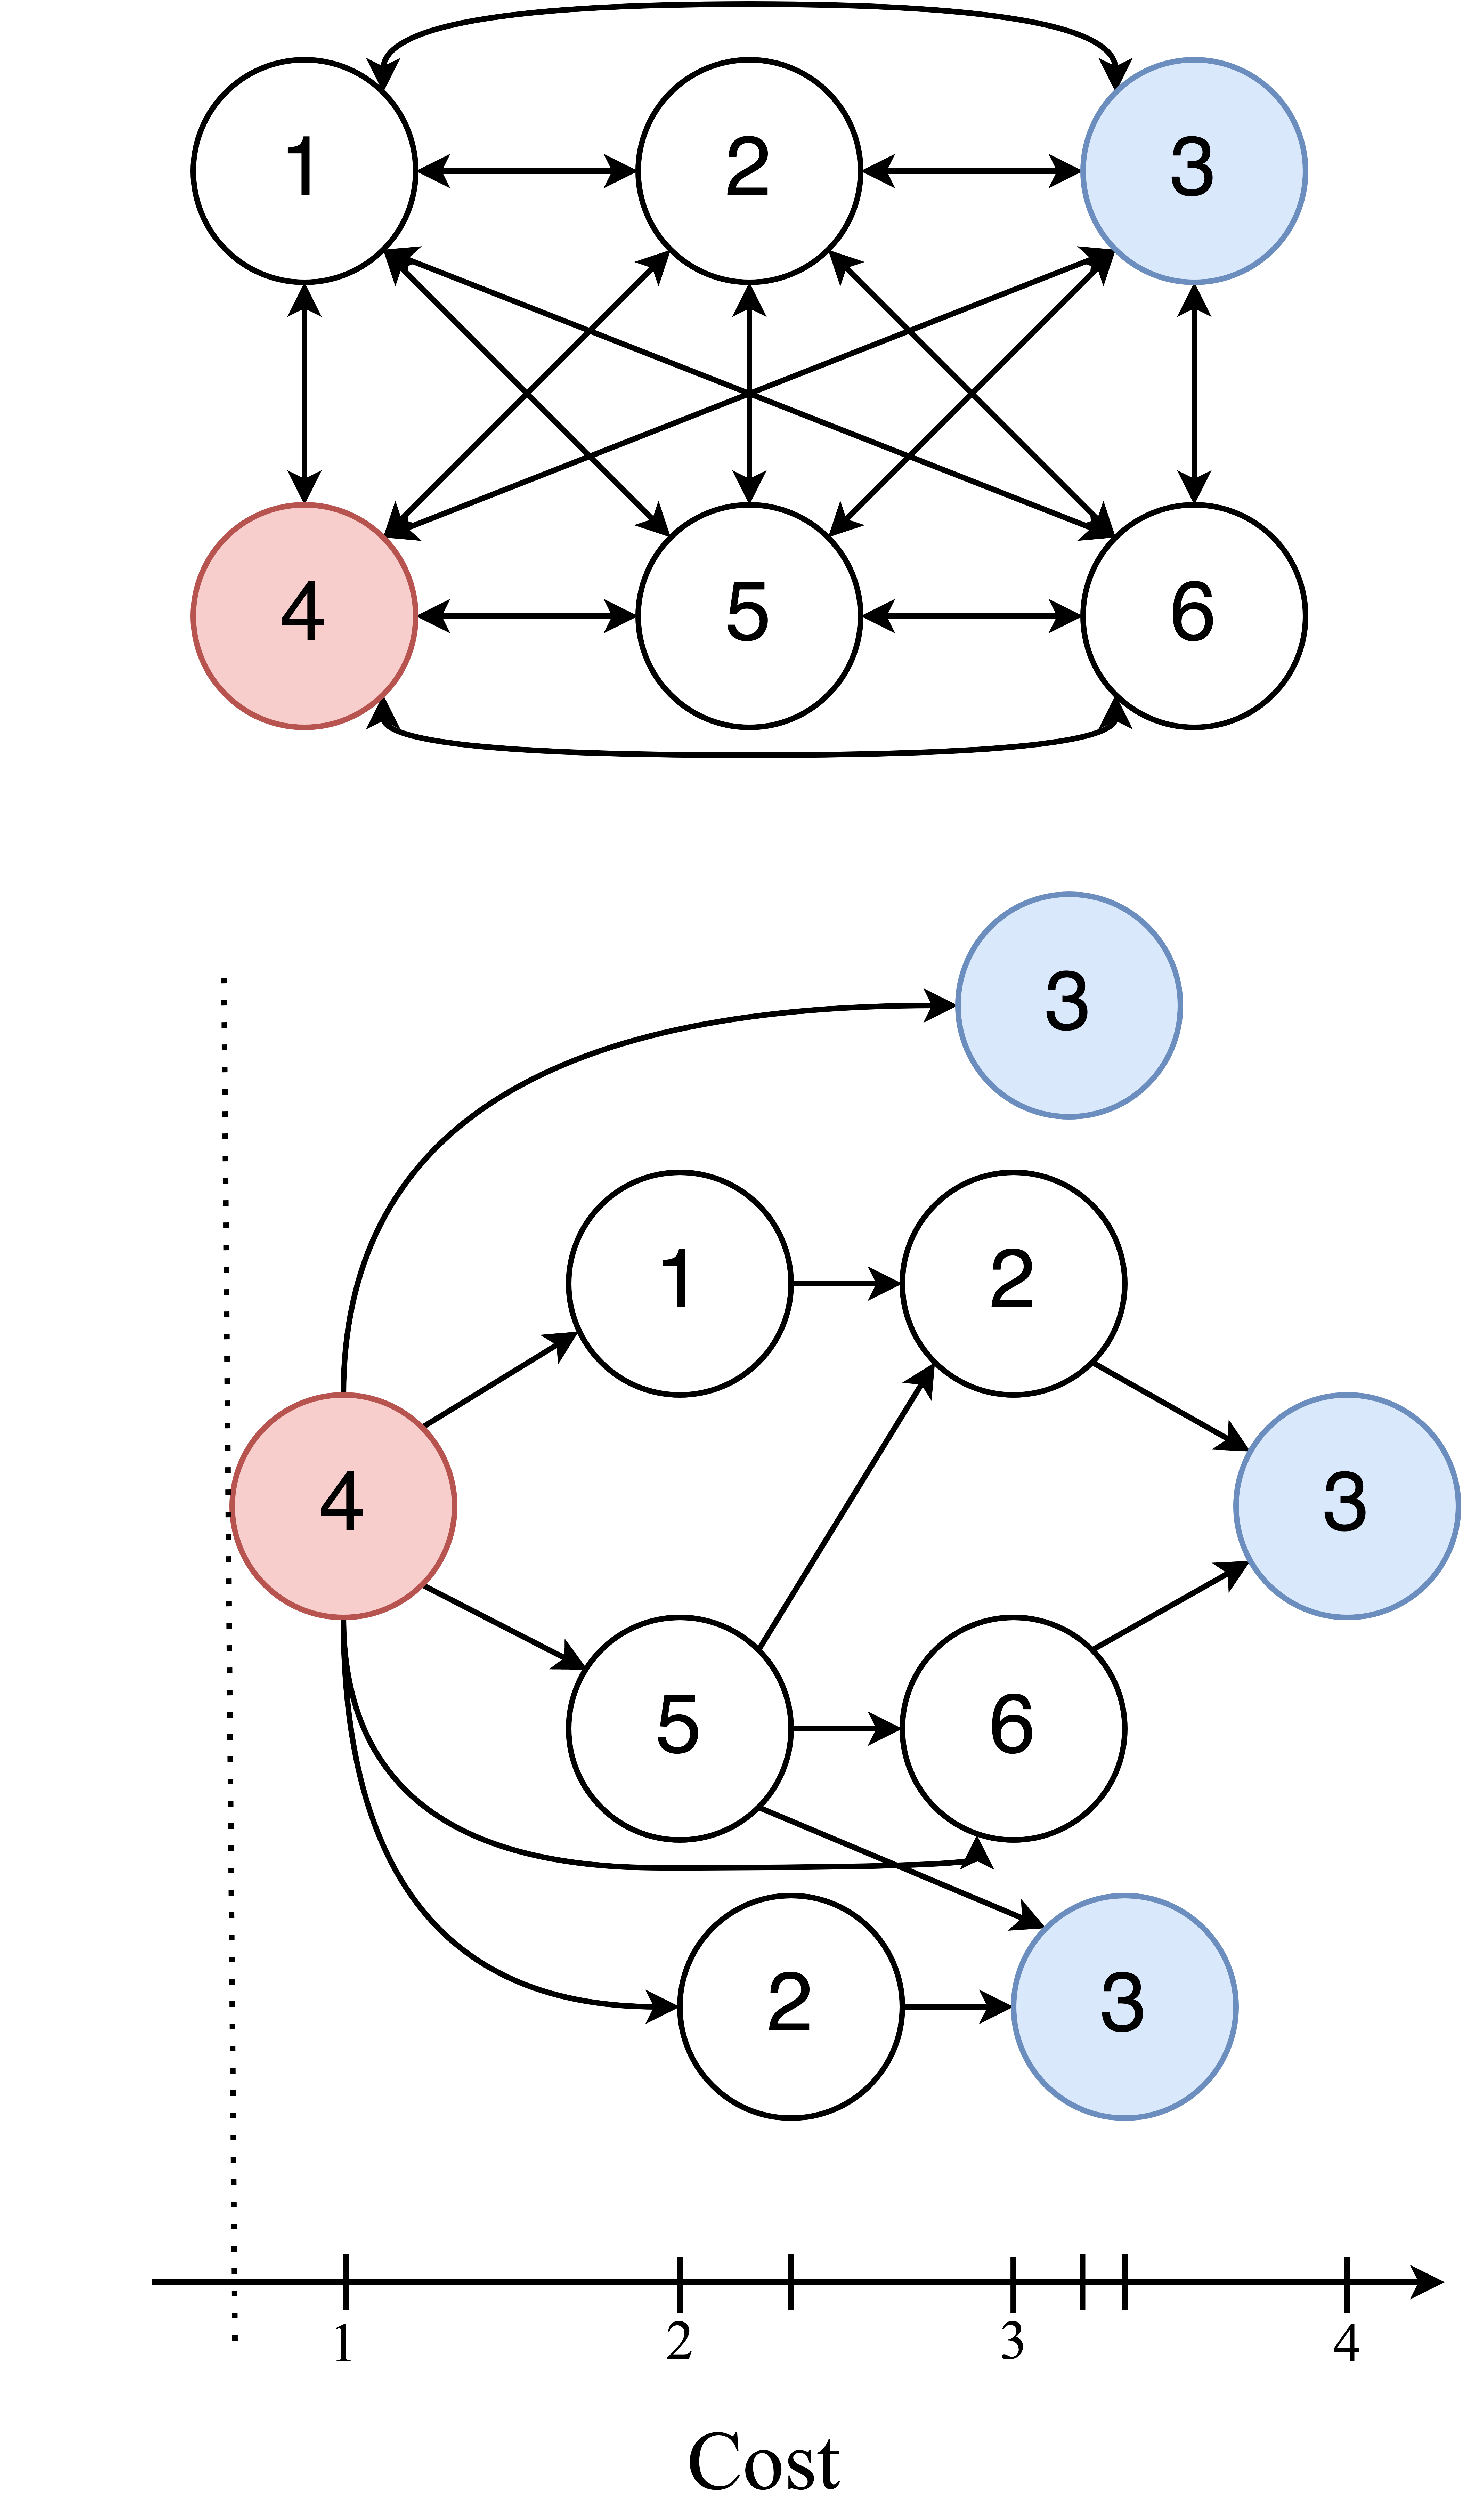
\includegraphics[width=0.7\linewidth]{ICTSNonUnit2}
    \caption{On the right, instead, we consider the variation in which the
      graph is fully connected, so there are some edges which weigh more than
      one. In particular, from the image on the right, it is possible to see 
      that the cost increment is one, then in the interval $[3-4]$ there are 3 
      different sinks for the goal position. In case the cost increment is 
      smaller, for example 0.5, the interval $[3,3.5]$ contains two sinks, 
      whereas the $[3.5,4]$ interval contains only one sink.}
  \end{subfigure}
  \caption{A comparison between \acrs{ICTS} for the classical \acrs{MAPF} and
    how the \acrs{MDD} is built for non unitary edges.}
  \label{fig:eICTS}
\end{figure}
